% !TeX root = ../main.tex

\chapter{Results}
\section{Taiwan Mandarin and Taiwan Southern Min tones under coarticulation}

\subsection{Tone contours}

Tone contours of Taiwan Mandarin and Taiwan Southern Min tones in carryover and anticipatory positions are shown in Appendix \ref{Appendix:ToneContours}.

\subsection{Directionalities and magnitudes of coarticulatory effects in the two languages}

Tonal coarticulation of Taiwan Mandarin and Taiwan Southern Min in carry-over and anticipatory positions respectively are shown in figures \ref{Figure:LMMCarryover} and \ref{Figure:LMMAnticipatory}. For both languages, in both positions, the ambient tones were shown to exert positive impacts on the target tones, that is, a high ambient tone raised, and a low ambient tone lowered the target tone. This meant that in both languages, both the carry-over and anticipatory effects were assimilatory. In terms of magnitudes, carry-over effects were found to be equally strong between the two languages, while the anticipatory effect in Taiwan Mandarin was found to be weaker than that in Taiwan Southern Min.
This was also reflected in within-language comparisons. In Taiwan Mandarin, the carry-over effect was stronger than the anticipatory effect, whereas in Taiwan Southern Min, the two effects were equally strong.

\begin{figure}[hbt!]
\centering
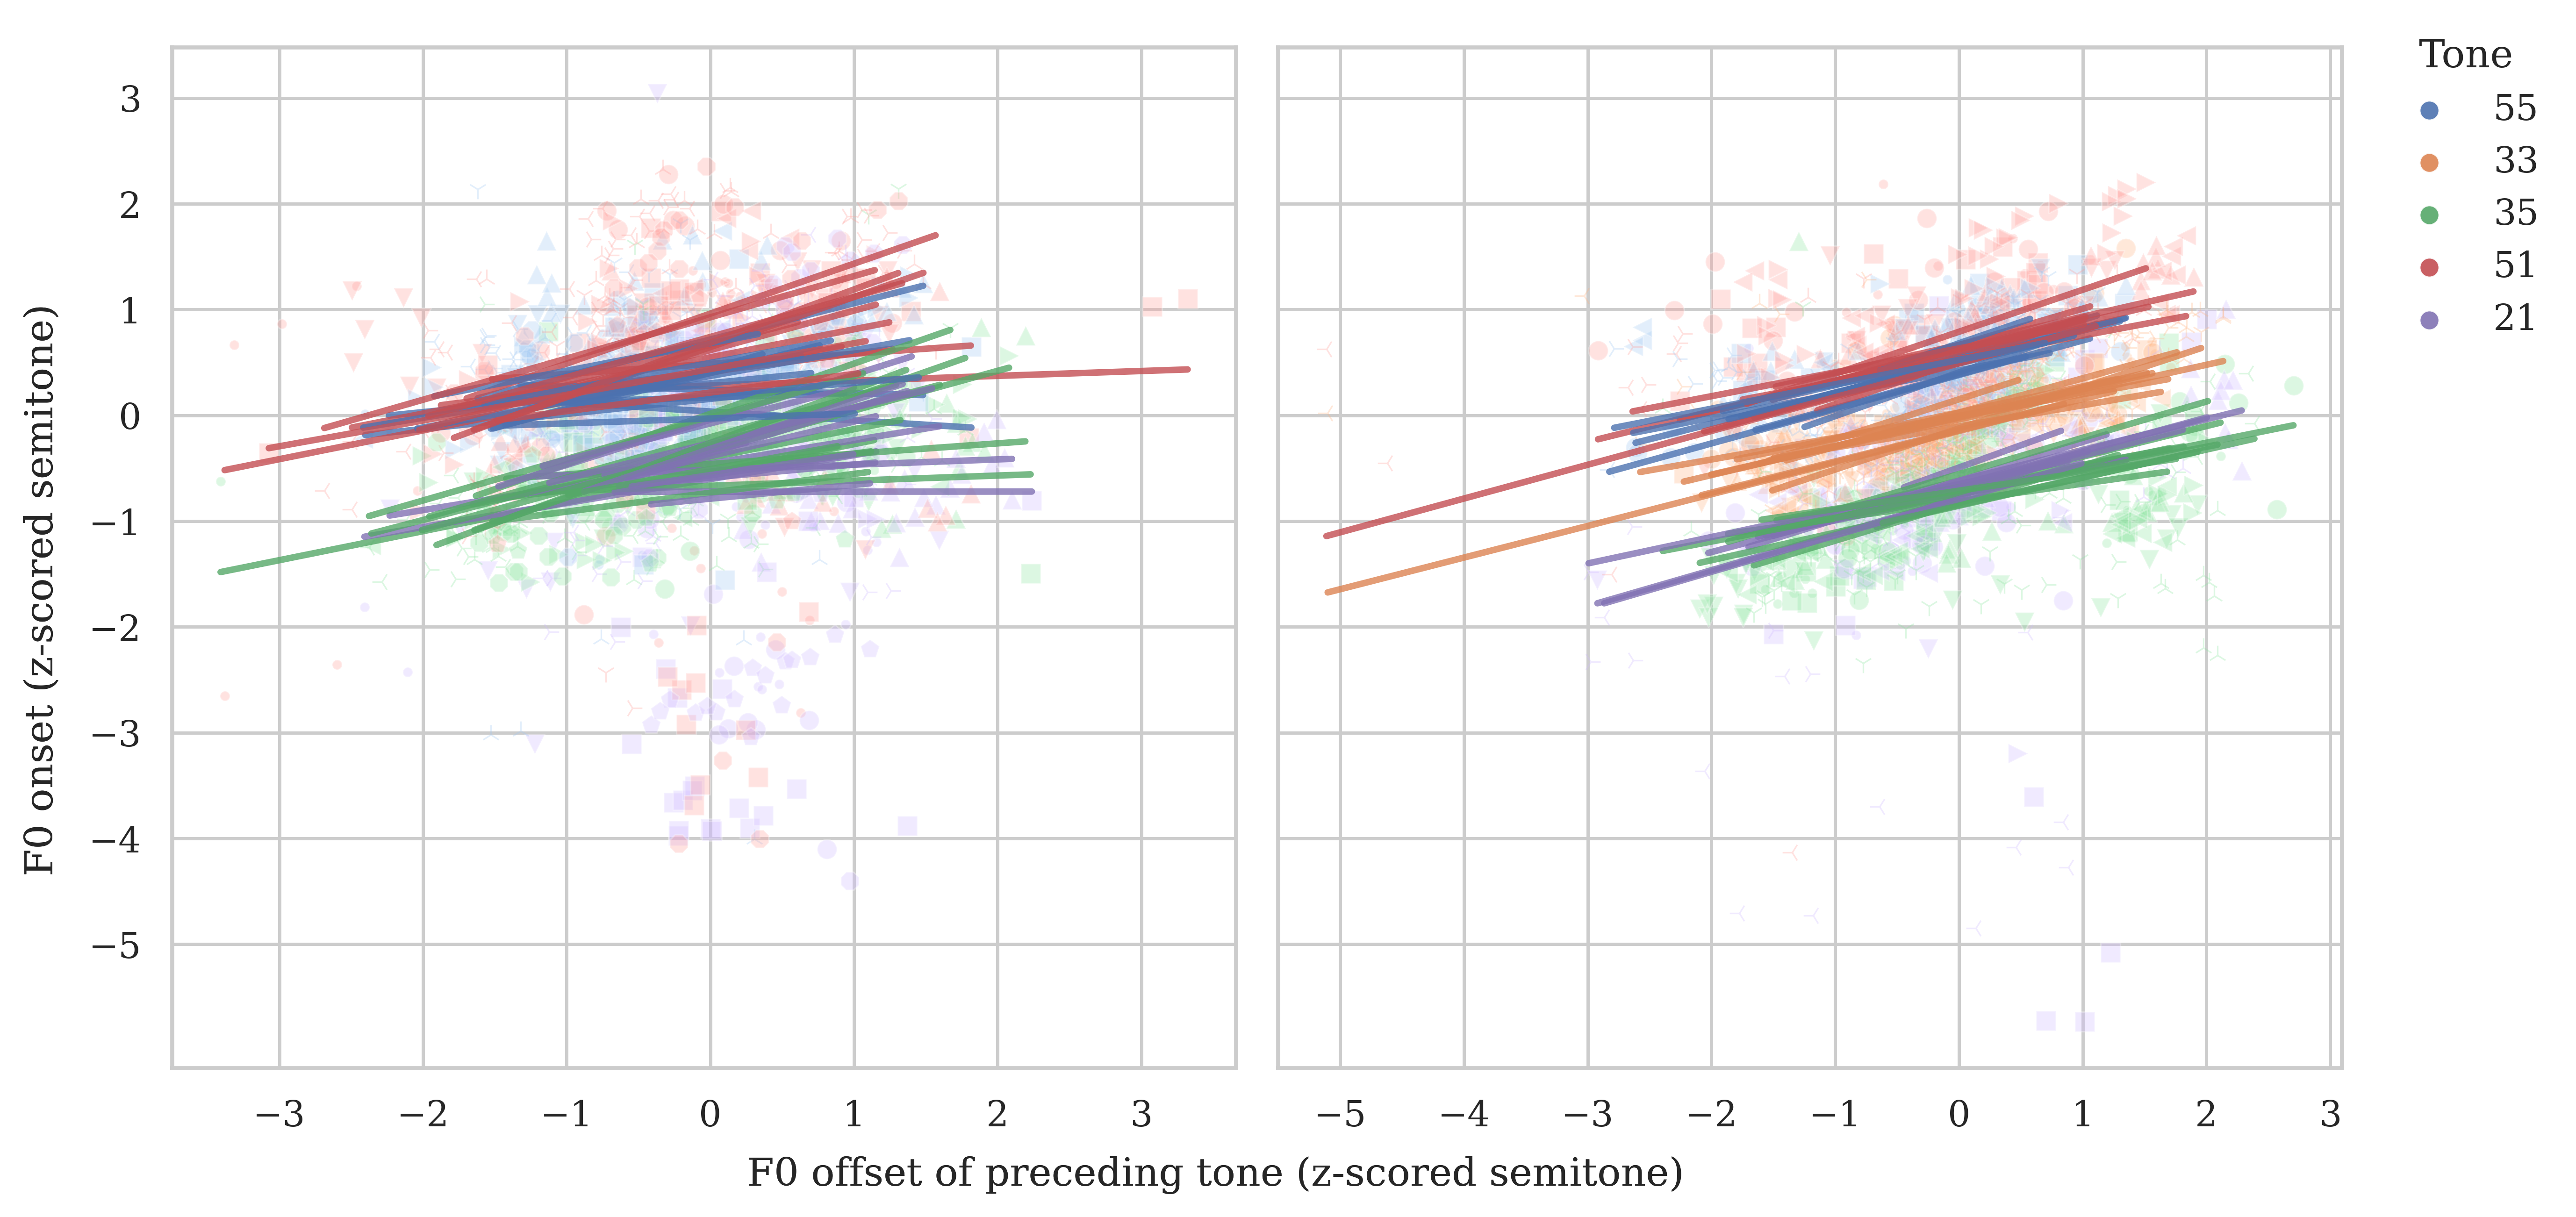
\includegraphics[width=\textwidth, trim={0 .5cm 0 0}]{figures/E1/Carryover_lang_seperated.png}
\caption{Fitted LMM model of tone onsets and offsets in carry-over positions (left: Taiwan Mandarin; right: Taiwan Southern Min).}
\label{Figure:LMMCarryover}
\end{figure}

\begin{figure}[hbt!]
\centering
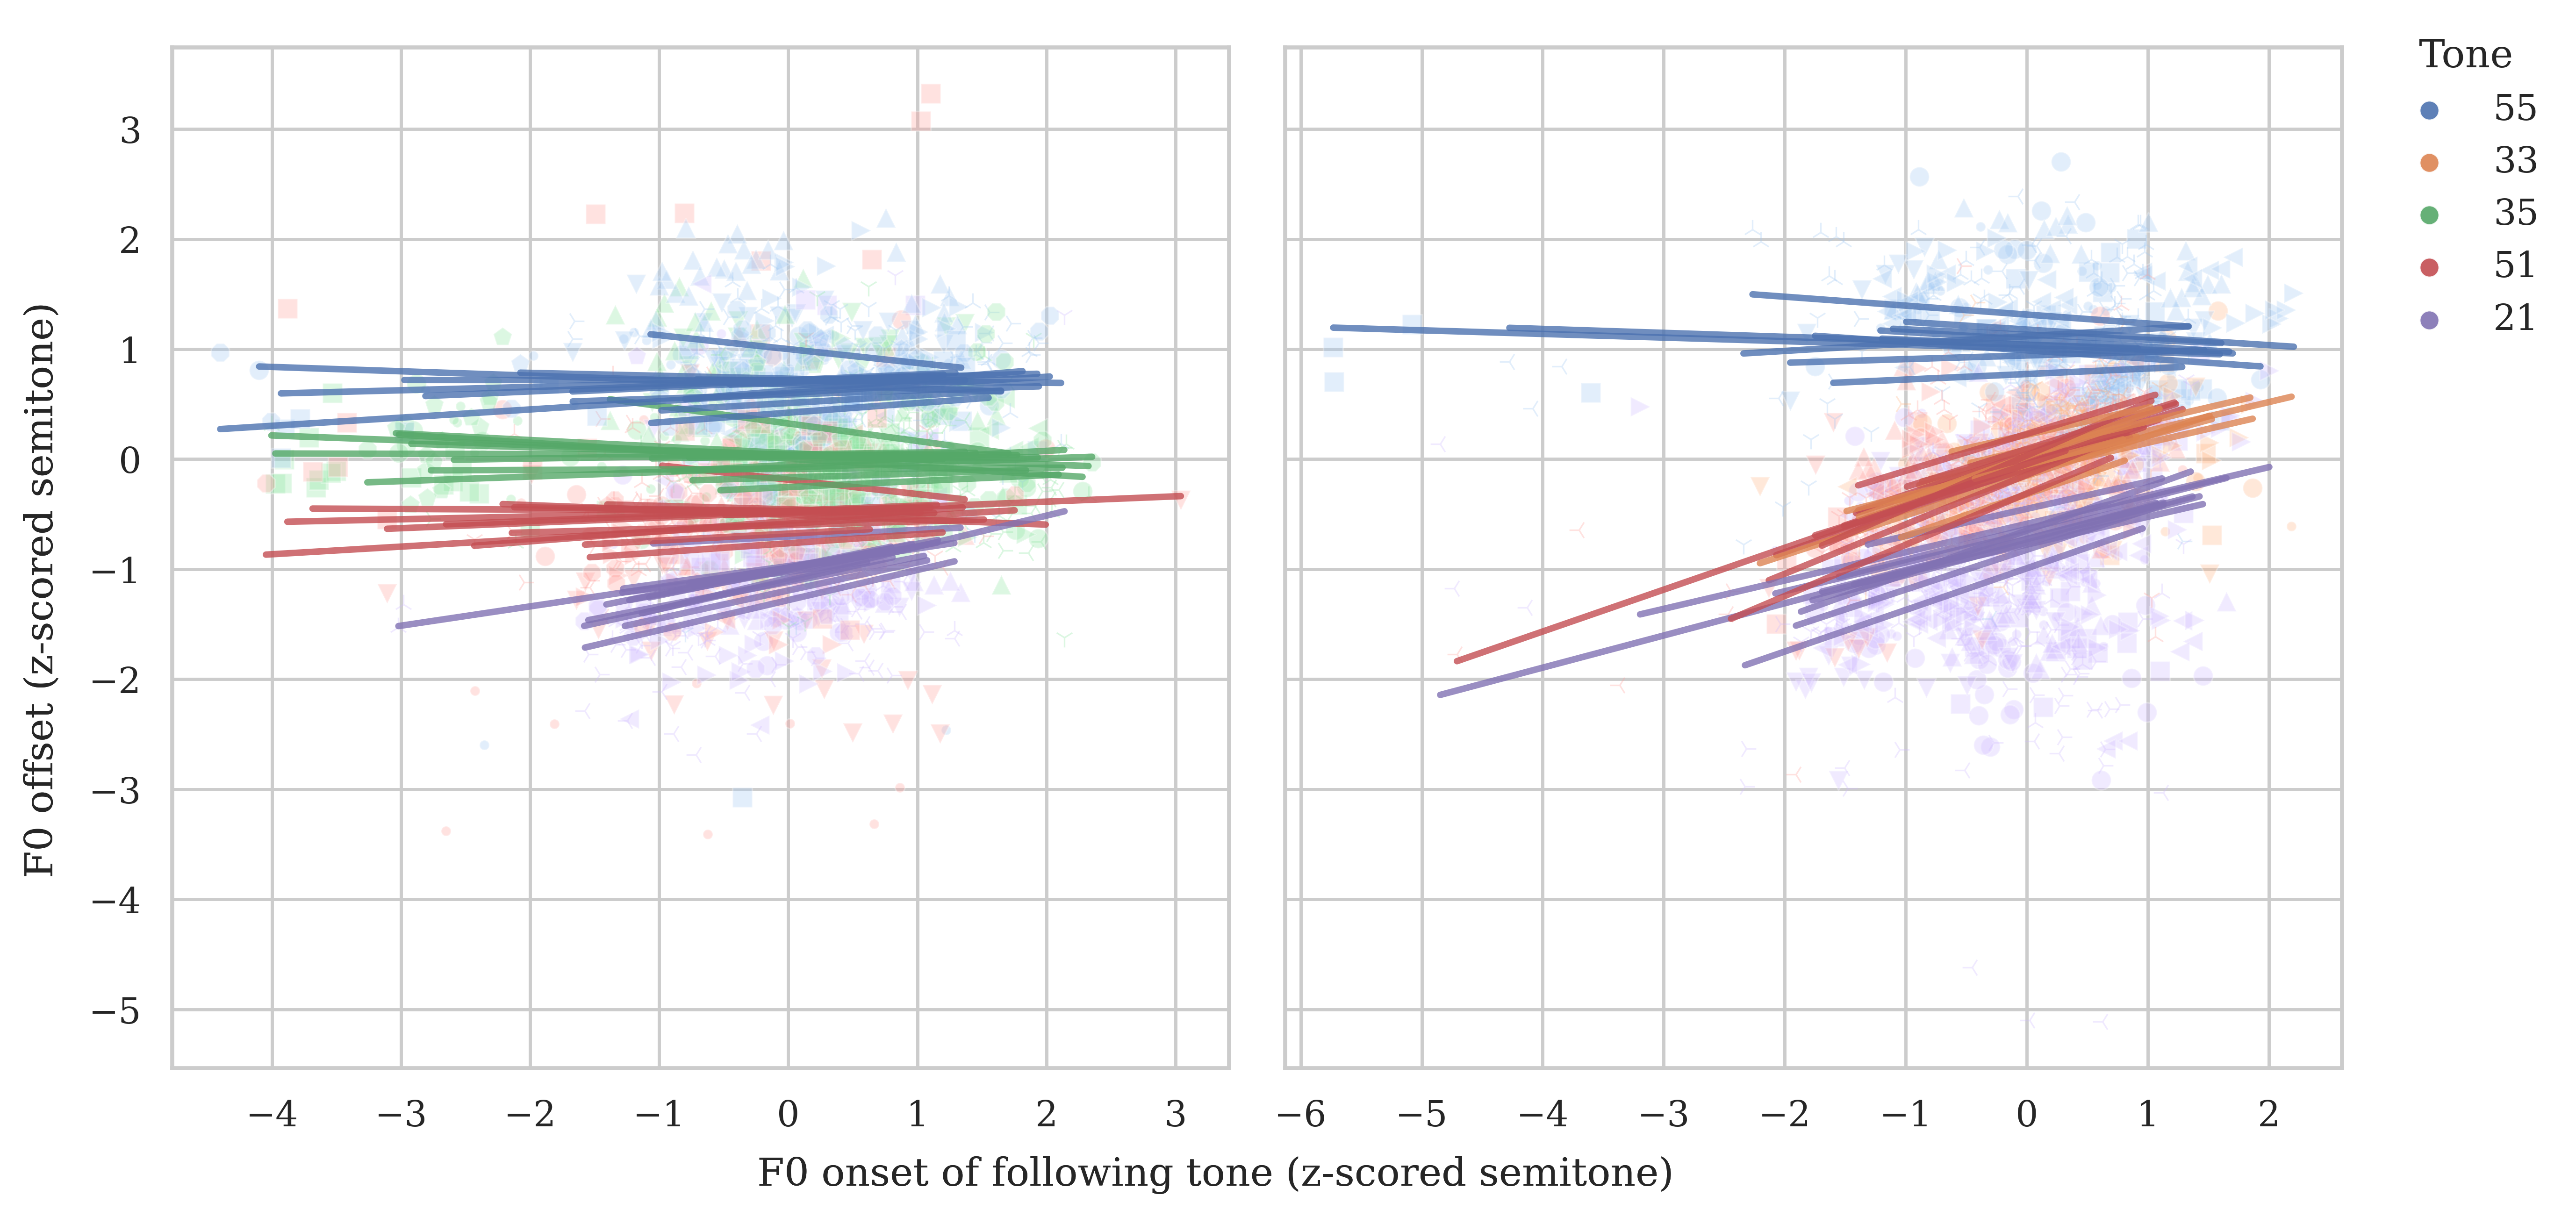
\includegraphics[width=\textwidth, trim={0 .5cm 0 0}]{figures/E1/Anticipatory_lang_seperated.png}
\caption{Fitted LMM model of tone onsets and offsets in anticipatory positions (left: Taiwan Mandarin; right: Taiwan Southern Min).}
\label{Figure:LMMAnticipatory}
\end{figure}

%\begin{figure}[hbt!]
%\centering
%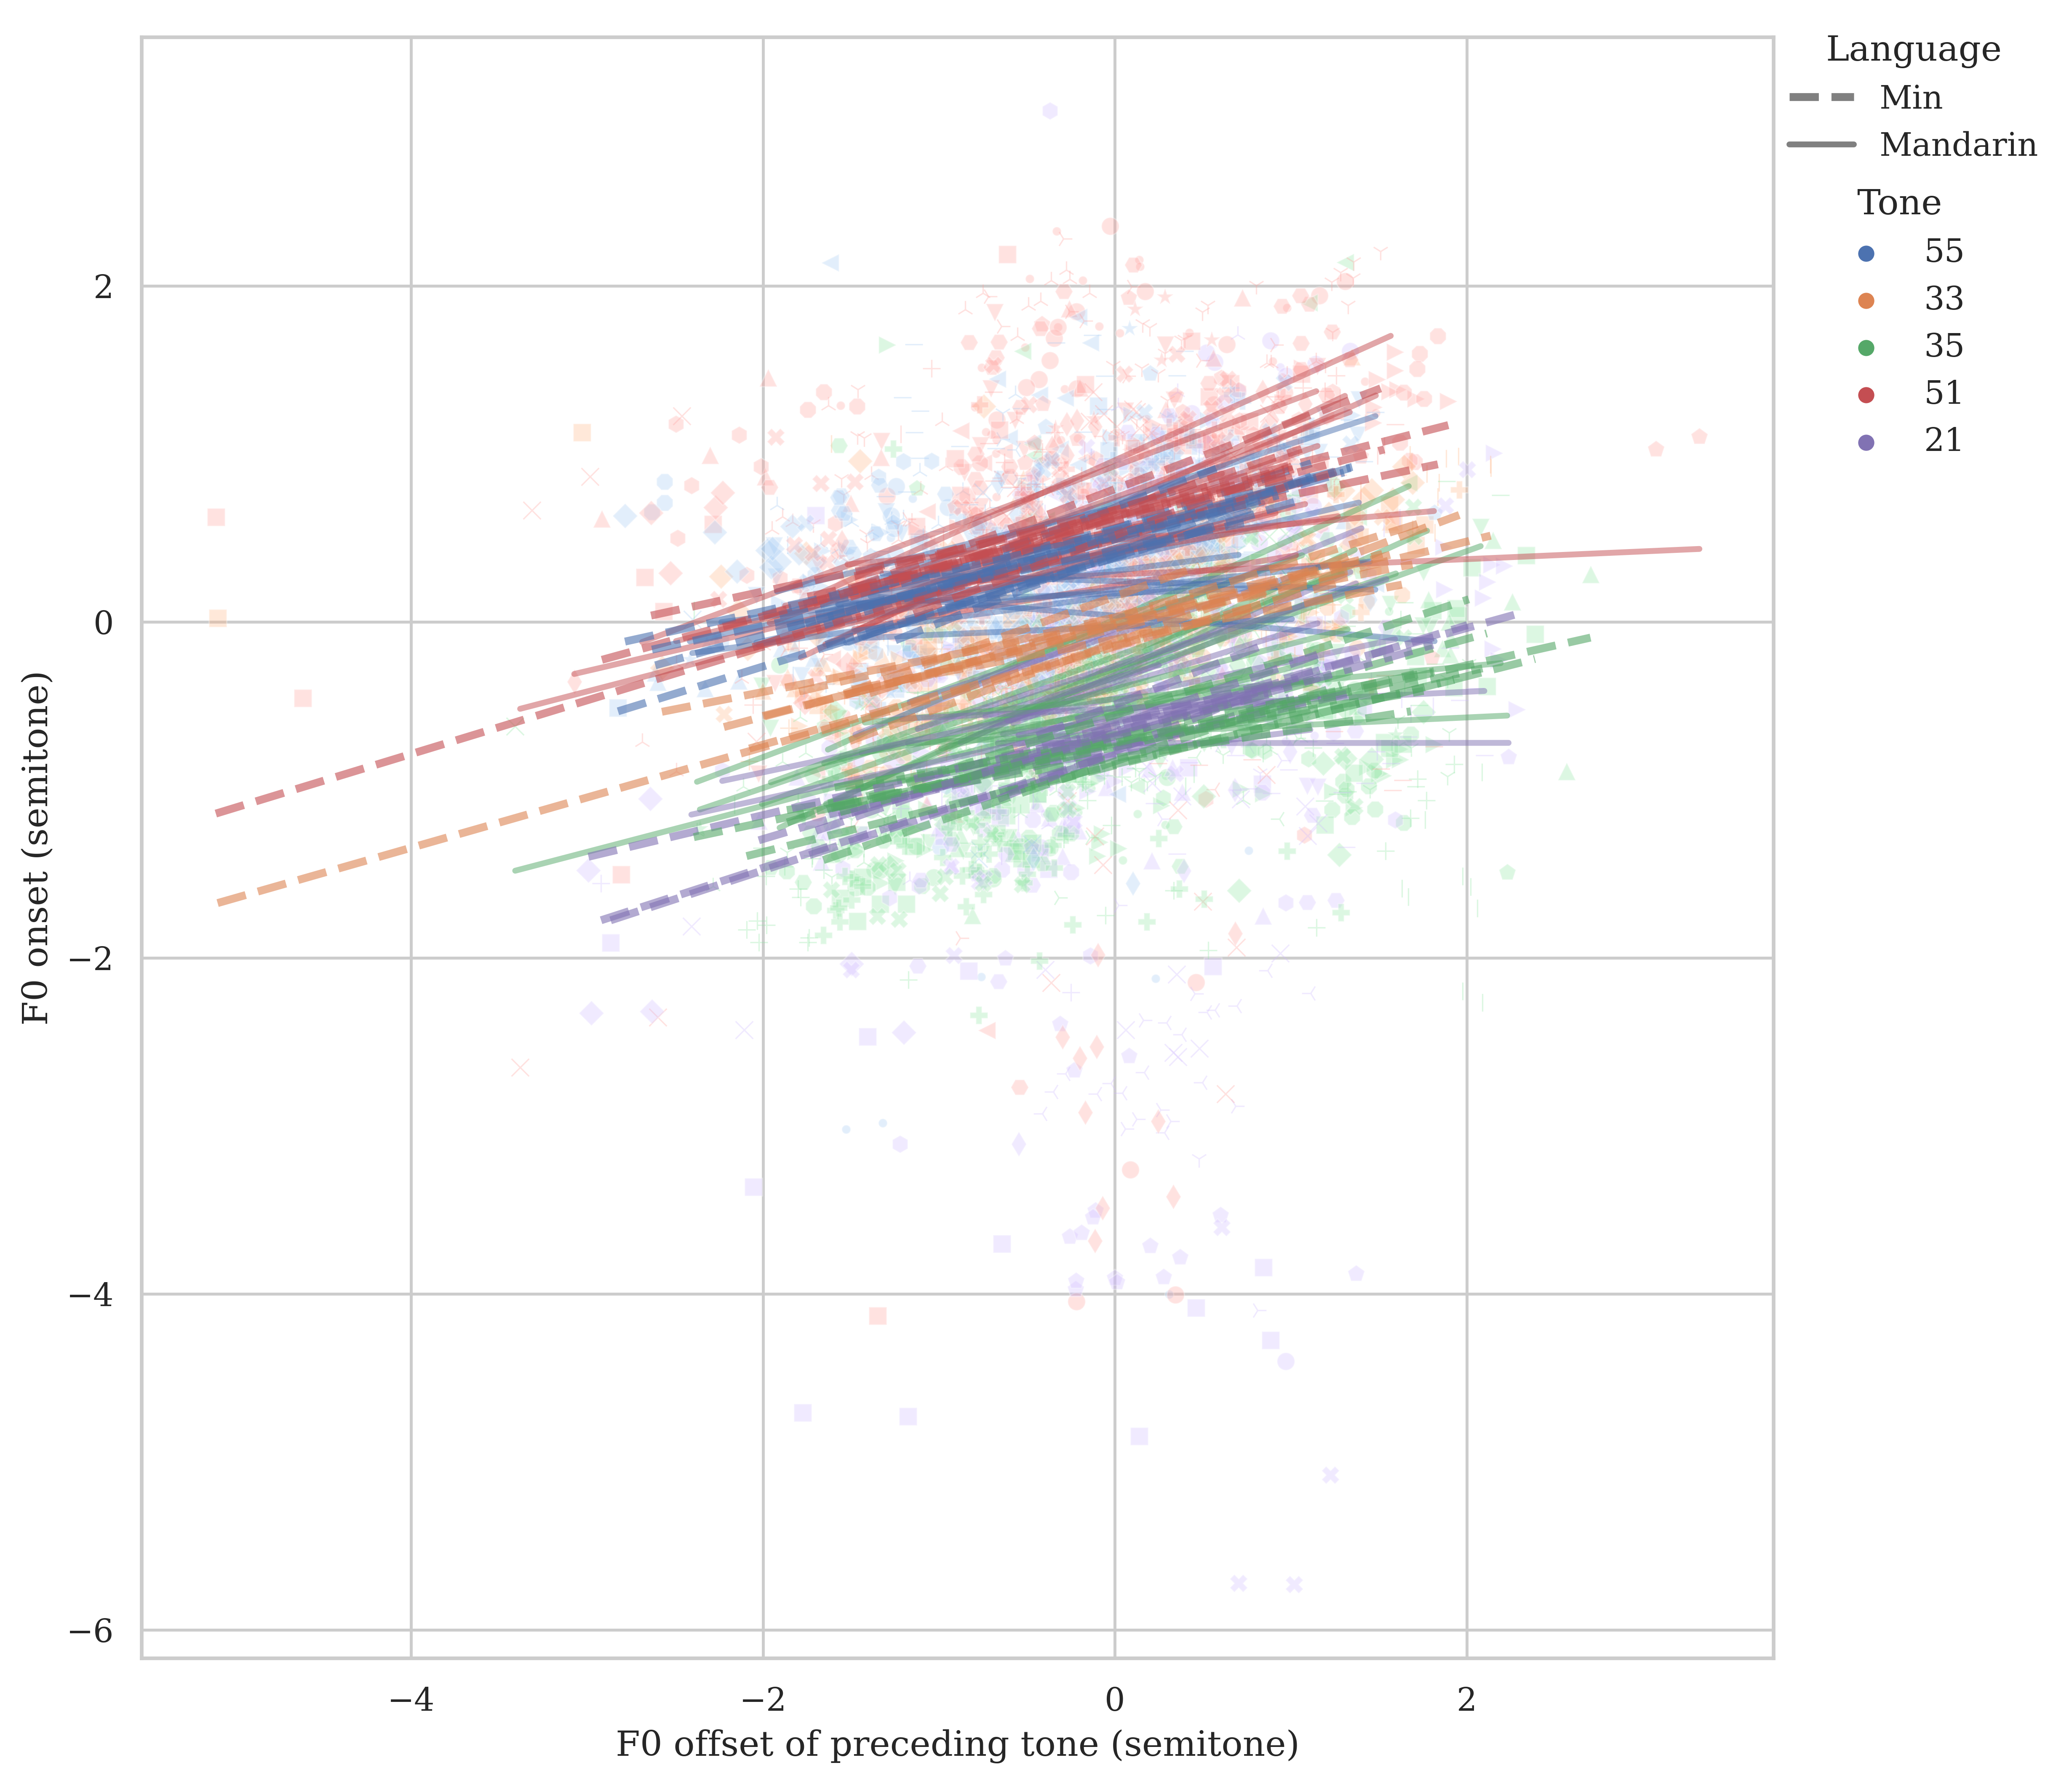
\includegraphics[scale=.45, trim={0 .5cm 0 0}]{figures/E1/Carryover.png}
%\caption{Fitted LMM model of tone onsets and offsets in carry-over positions.}
%\label{Figure:LMMCarryover}
%\end{figure}
%
%\begin{figure}[hbt!]
%\centering
%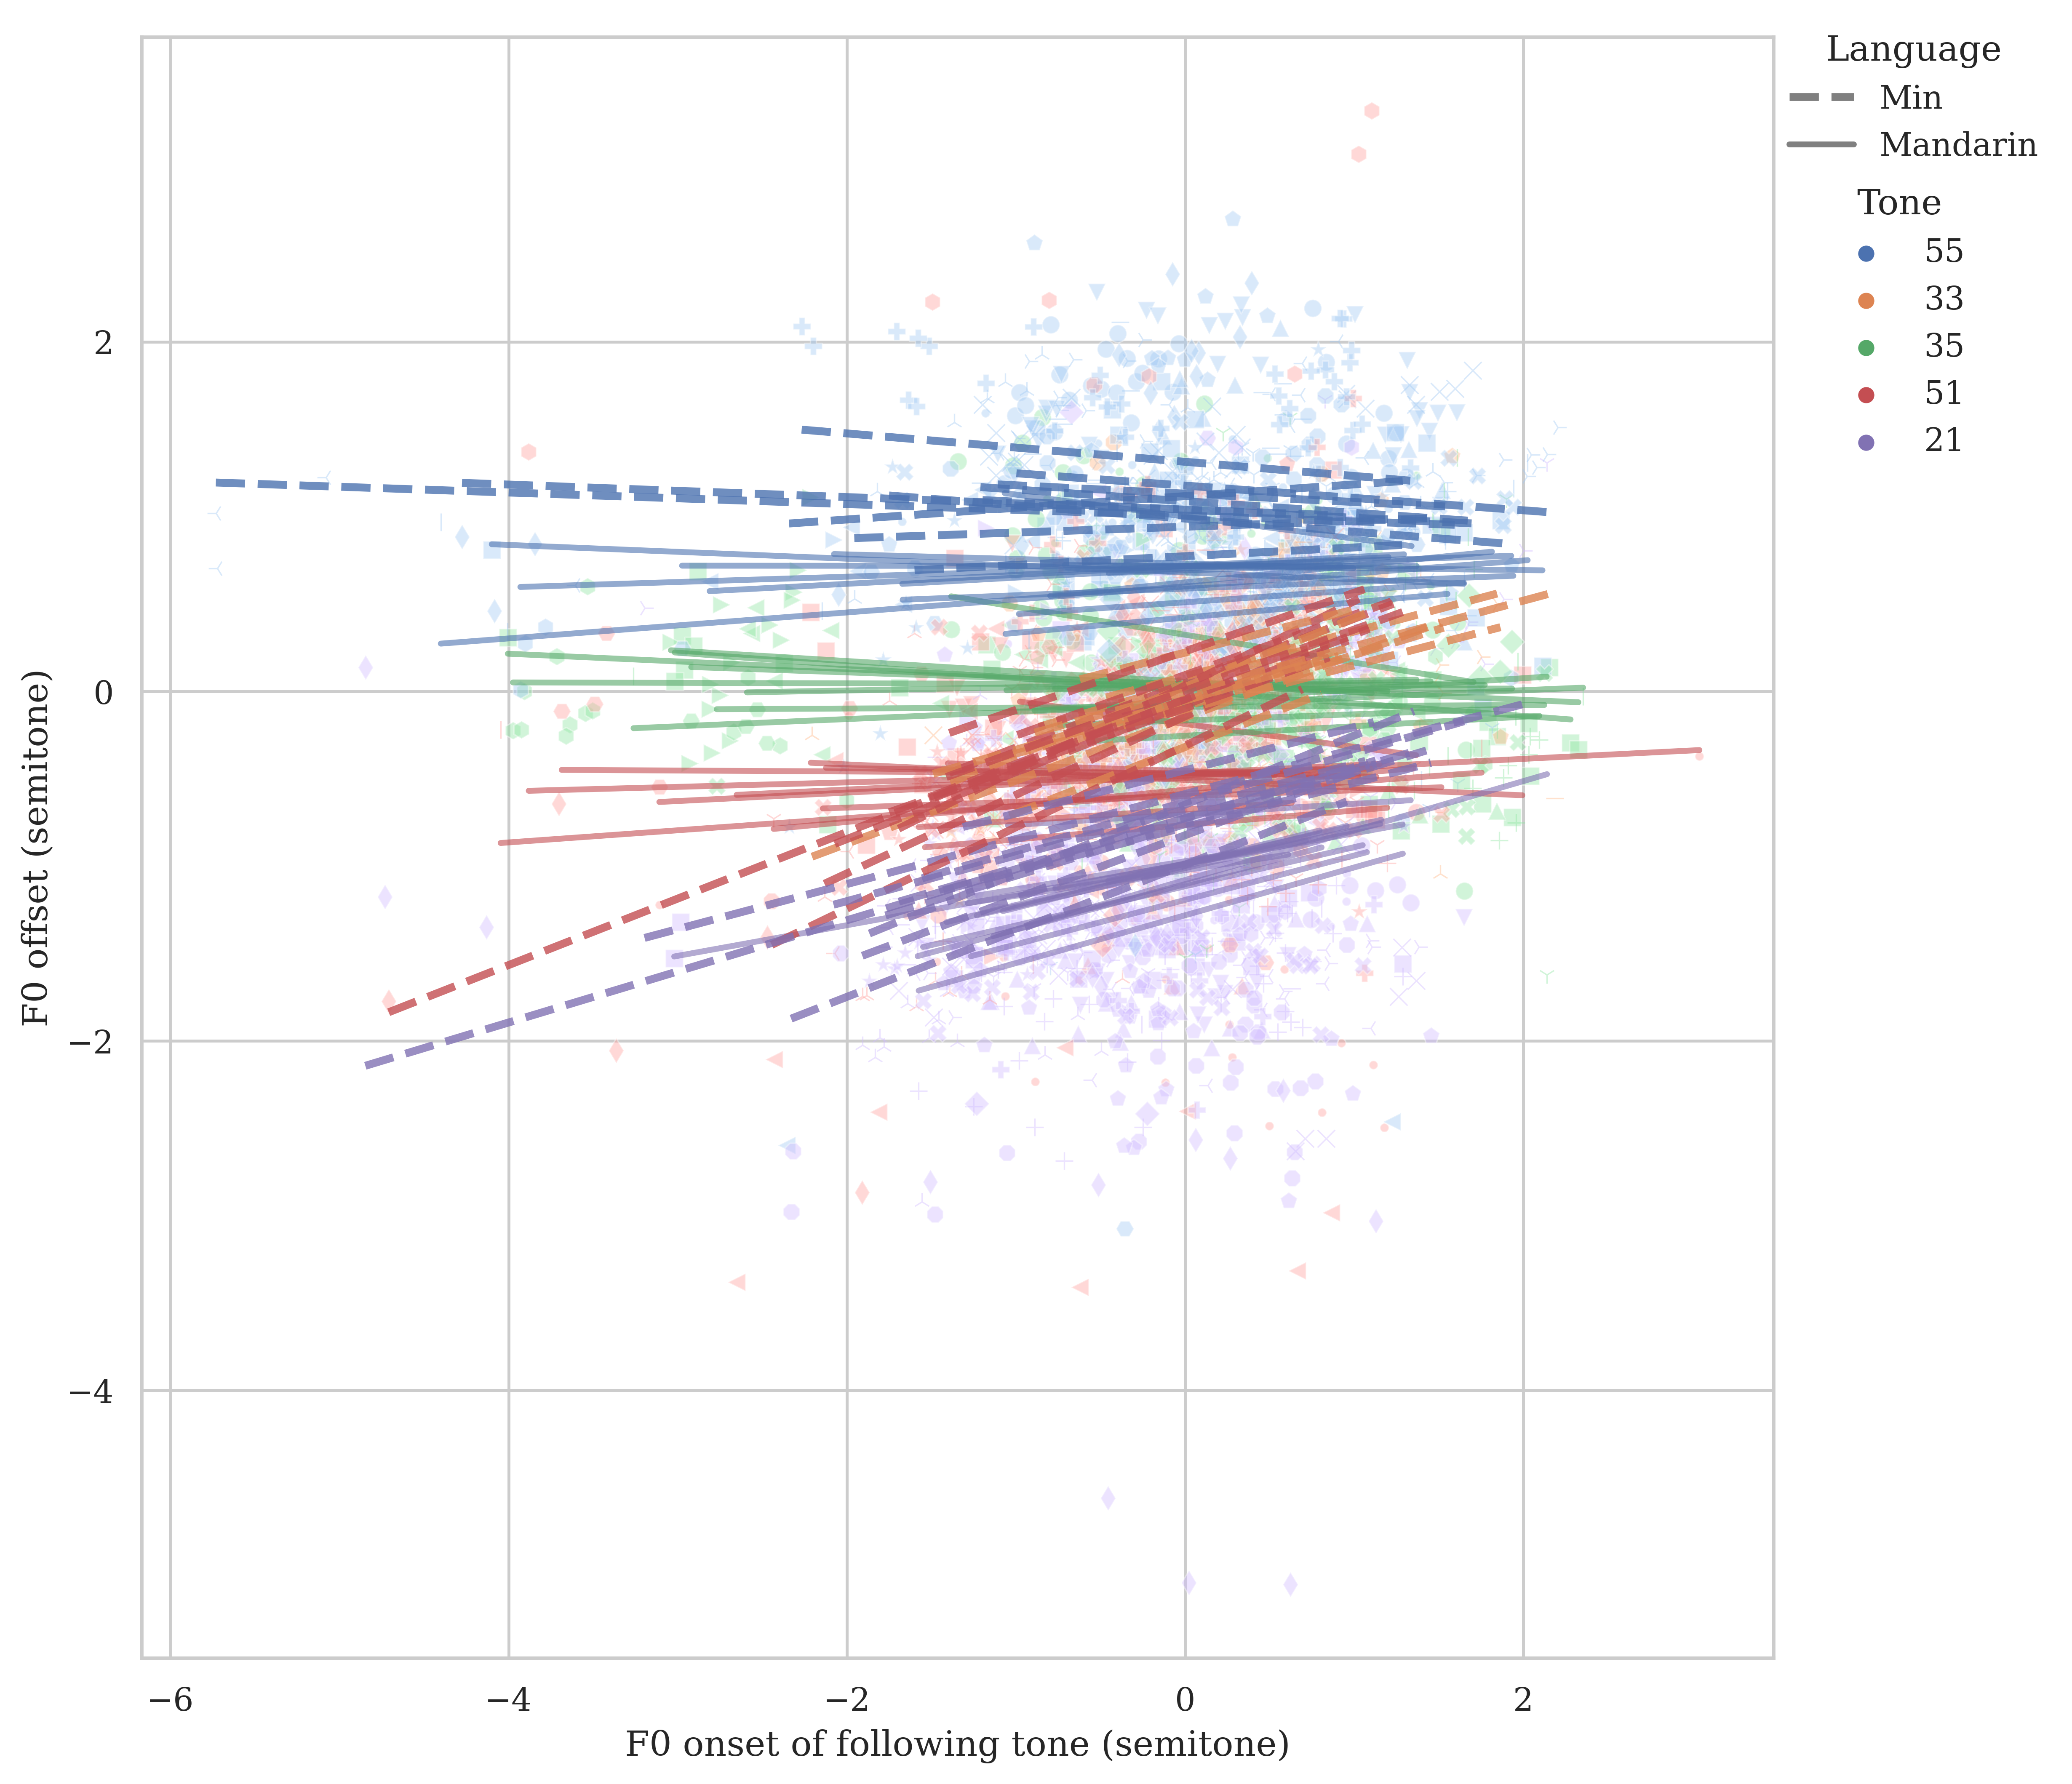
\includegraphics[scale=.45, trim={0 .5cm 0 0}]{figures/E1/Anticipatory.png}
%\caption{Fitted LMM model of tone onsets and offsets in anticipatory positions.}
%\label{Figure:LMMAnticipatory}
%\end{figure}

In general, tonal coarticulation in Taiwan Mandarin and Taiwan Southern Min were almost identical in both directionality and magnitudes. Symmetries were found in both languages, and no difference of magnitude was found. This can be summarized in tables \ref{table:MandarinDistribution} to \ref{table:MandarinMinDistributionComparison}.

\begin{flushleft}
\begin{table}[hbt!]
\begin{tabularx}{\textwidth}{l|X|X|}
\cline{2-3}
 & Magnitude & Direction \\
%\hhline{-::==}
\hhline{~|--}\noalign{\vspace*{\doublerulesep}}
\hhline{-||--}
\multicolumn{1}{|X||}{Carry-over} & Stronger & \multirow{2}{*}{Assimilatory}\\
\hhline{|-||-~}
\multicolumn{1}{|X||}{Anticipatory} & Weaker& \\
\hhline{|-||-|-|}
\end{tabularx}
\caption{Distribution of tonal coarticulation in Taiwan Mandarin}
\label{table:MandarinDistribution}
\end{table}
\end{flushleft}

\begin{flushleft}
\begin{table}[hbt!]
\begin{tabularx}{\textwidth}{l|X|X|}
\cline{2-3}
 & Magnitude & Direction \\
%\hhline{-::==}
\hhline{~|--}\noalign{\vspace*{\doublerulesep}}
\hhline{-||--}
\multicolumn{1}{|X||}{Carry-over} & \multirow{2}{*}{Equally strong} & \multirow{2}{*}{Assimilatory}\\
\hhline{|-||~~}
\multicolumn{1}{|X||}{Anticipatory} &  & \\
\hhline{|-||-|-|}
\end{tabularx}
\caption{Distribution of tonal coarticulation in Taiwan Southern Min}
\label{table:MinDistribution}
\end{table}
\end{flushleft}

\begin{flushleft}
\begin{table}[hbt!]
\begin{tabularx}{\textwidth}{l|X|X|}
\cline{2-3}
 & Carry-over & Anticipatory \\
\hhline{~|--}\noalign{\vspace*{\doublerulesep}}
\hhline{-||--}
\multicolumn{1}{|X||}{Taiwan Mandarin} & \multirow{2}{*}{Equally strong} & Weaker\\
\hhline{|-||~-}
\multicolumn{1}{|X||}{Taiwan Southern Min} &  & Stronger\\
\hhline{|-||-|-|}
\end{tabularx}
\caption{Comparison of tonal coarticulation between Taiwan Mandarin and Taiwan Southern Min}
\label{table:MandarinMinDistributionComparison}
\end{table}
\end{flushleft}

\section{Normalization for tonal coarticulation in Taiwan Mandarin and Taiwan Southern Min}
Raw falling tone responses of the the monolingual and bilingual groups in Mandarin and Southern Min are shown in Figure \ref{Figure:E2Raw}.

\begin{figure}[hbt!]
\centering
\begin{subfigure}[b]{.45\textwidth}
\centering
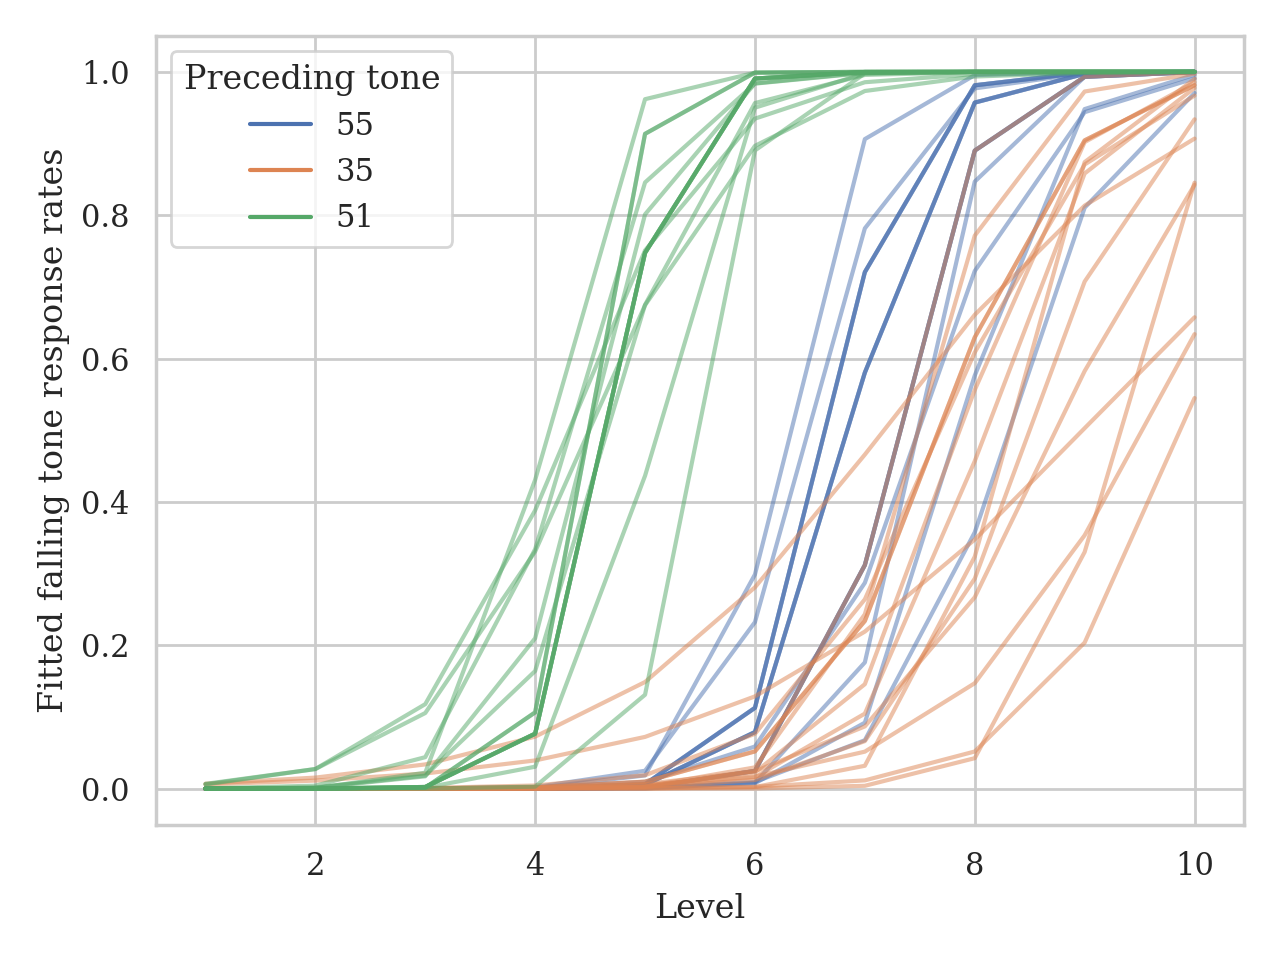
\includegraphics[width=\textwidth]{figures/E2/Mandarin_monolingual_E2_raw.png}
\end{subfigure}
\hfill
\begin{subfigure}[b]{.45\textwidth}
\centering
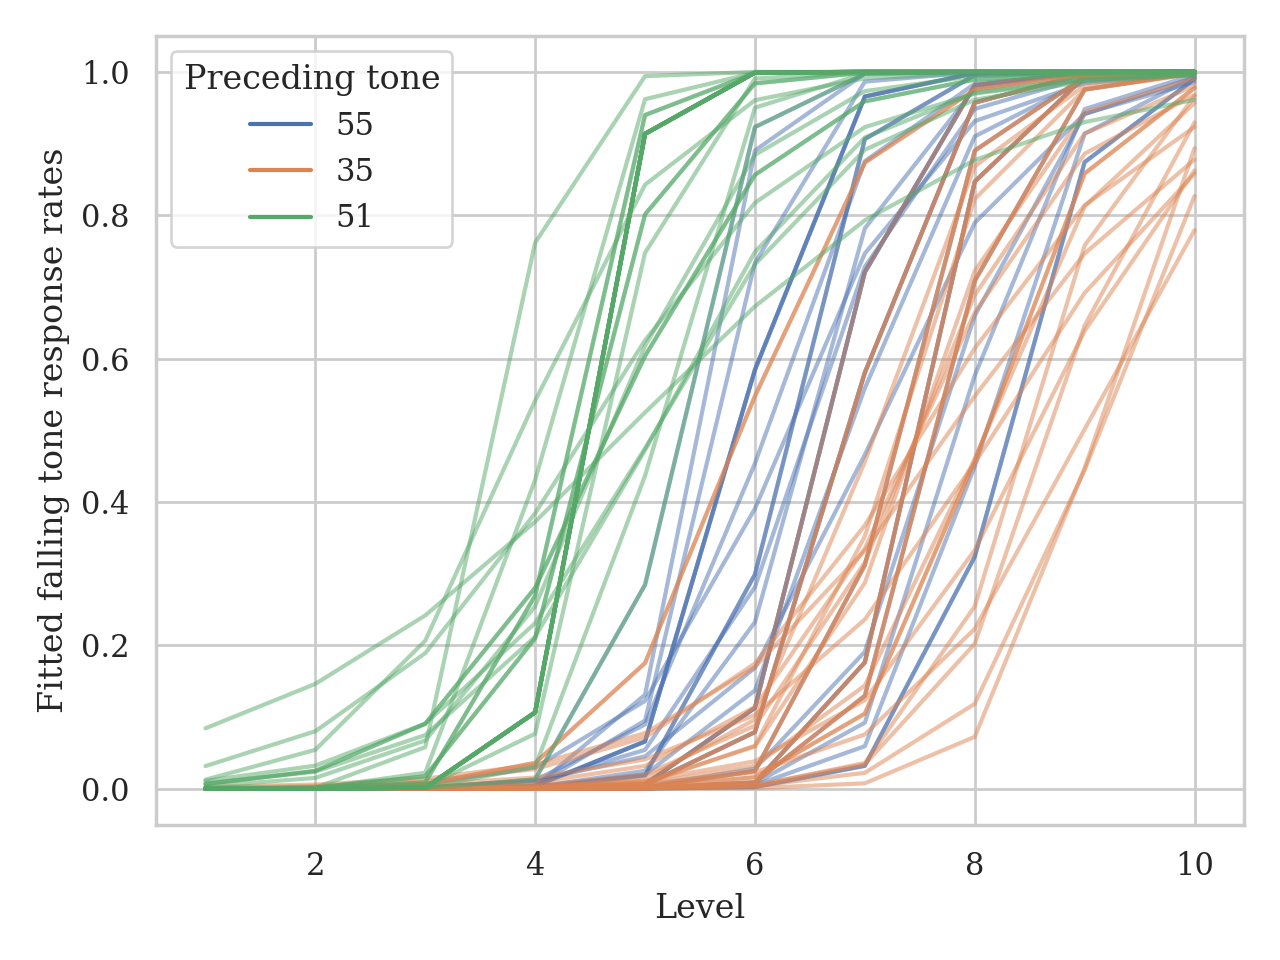
\includegraphics[width=\textwidth]{figures/E2/Mandarin_bilingual_E2_raw.png}
\end{subfigure}
\hfill
\begin{subfigure}[b]{.45\textwidth}
\centering
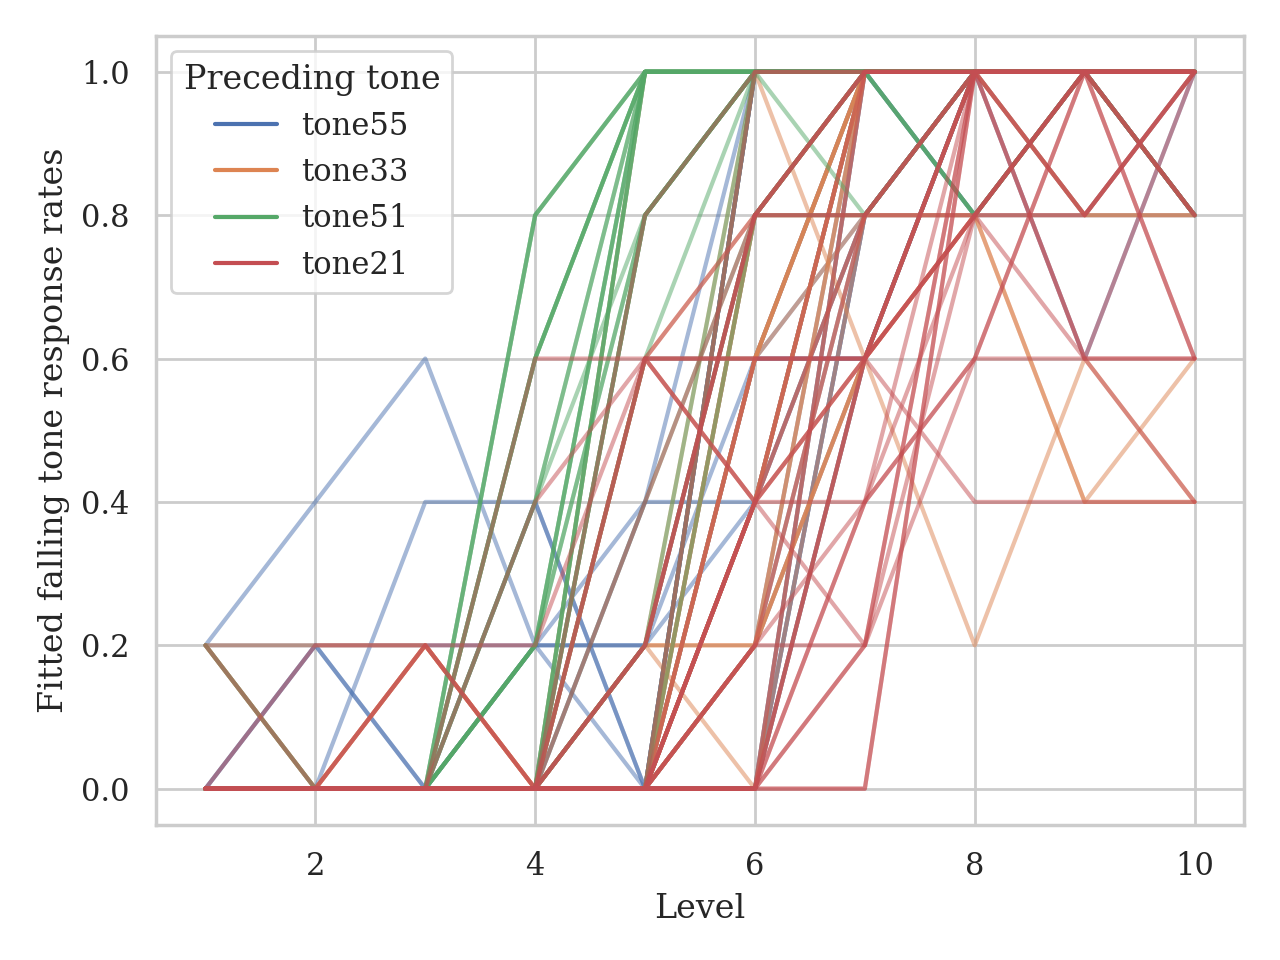
\includegraphics[width=\textwidth]{figures/E2/Min_E2_raw.png}
\end{subfigure}
\caption{Falling tone response percentages in Experiment 2 (top left: Mandarin (monolingual); top right: Mandarin (bilingual); bottom: Southern Min).}
\label{Figure:E2Raw}
\end{figure}

Upon first sight, we see an obvious difference between the monolingual group's Mandarin results and the bilingual group's Southern Min results, with the latter being generally narrower. As shown in Figure \ref{Figure:E2GAMM}, the distances between the GAMM fitted splines of the monolingual group's Taiwan Mandarin falling tone responses were apparently wider than those in Taiwan Southern Min, and this linguistic difference was seen even within the bilingual group, where the distances between the splines of the bilingual group's Taiwan Mandarin results were also wider.

\begin{figure}[hbt!]
\centering
\begin{subfigure}[b]{.45\textwidth}
\centering
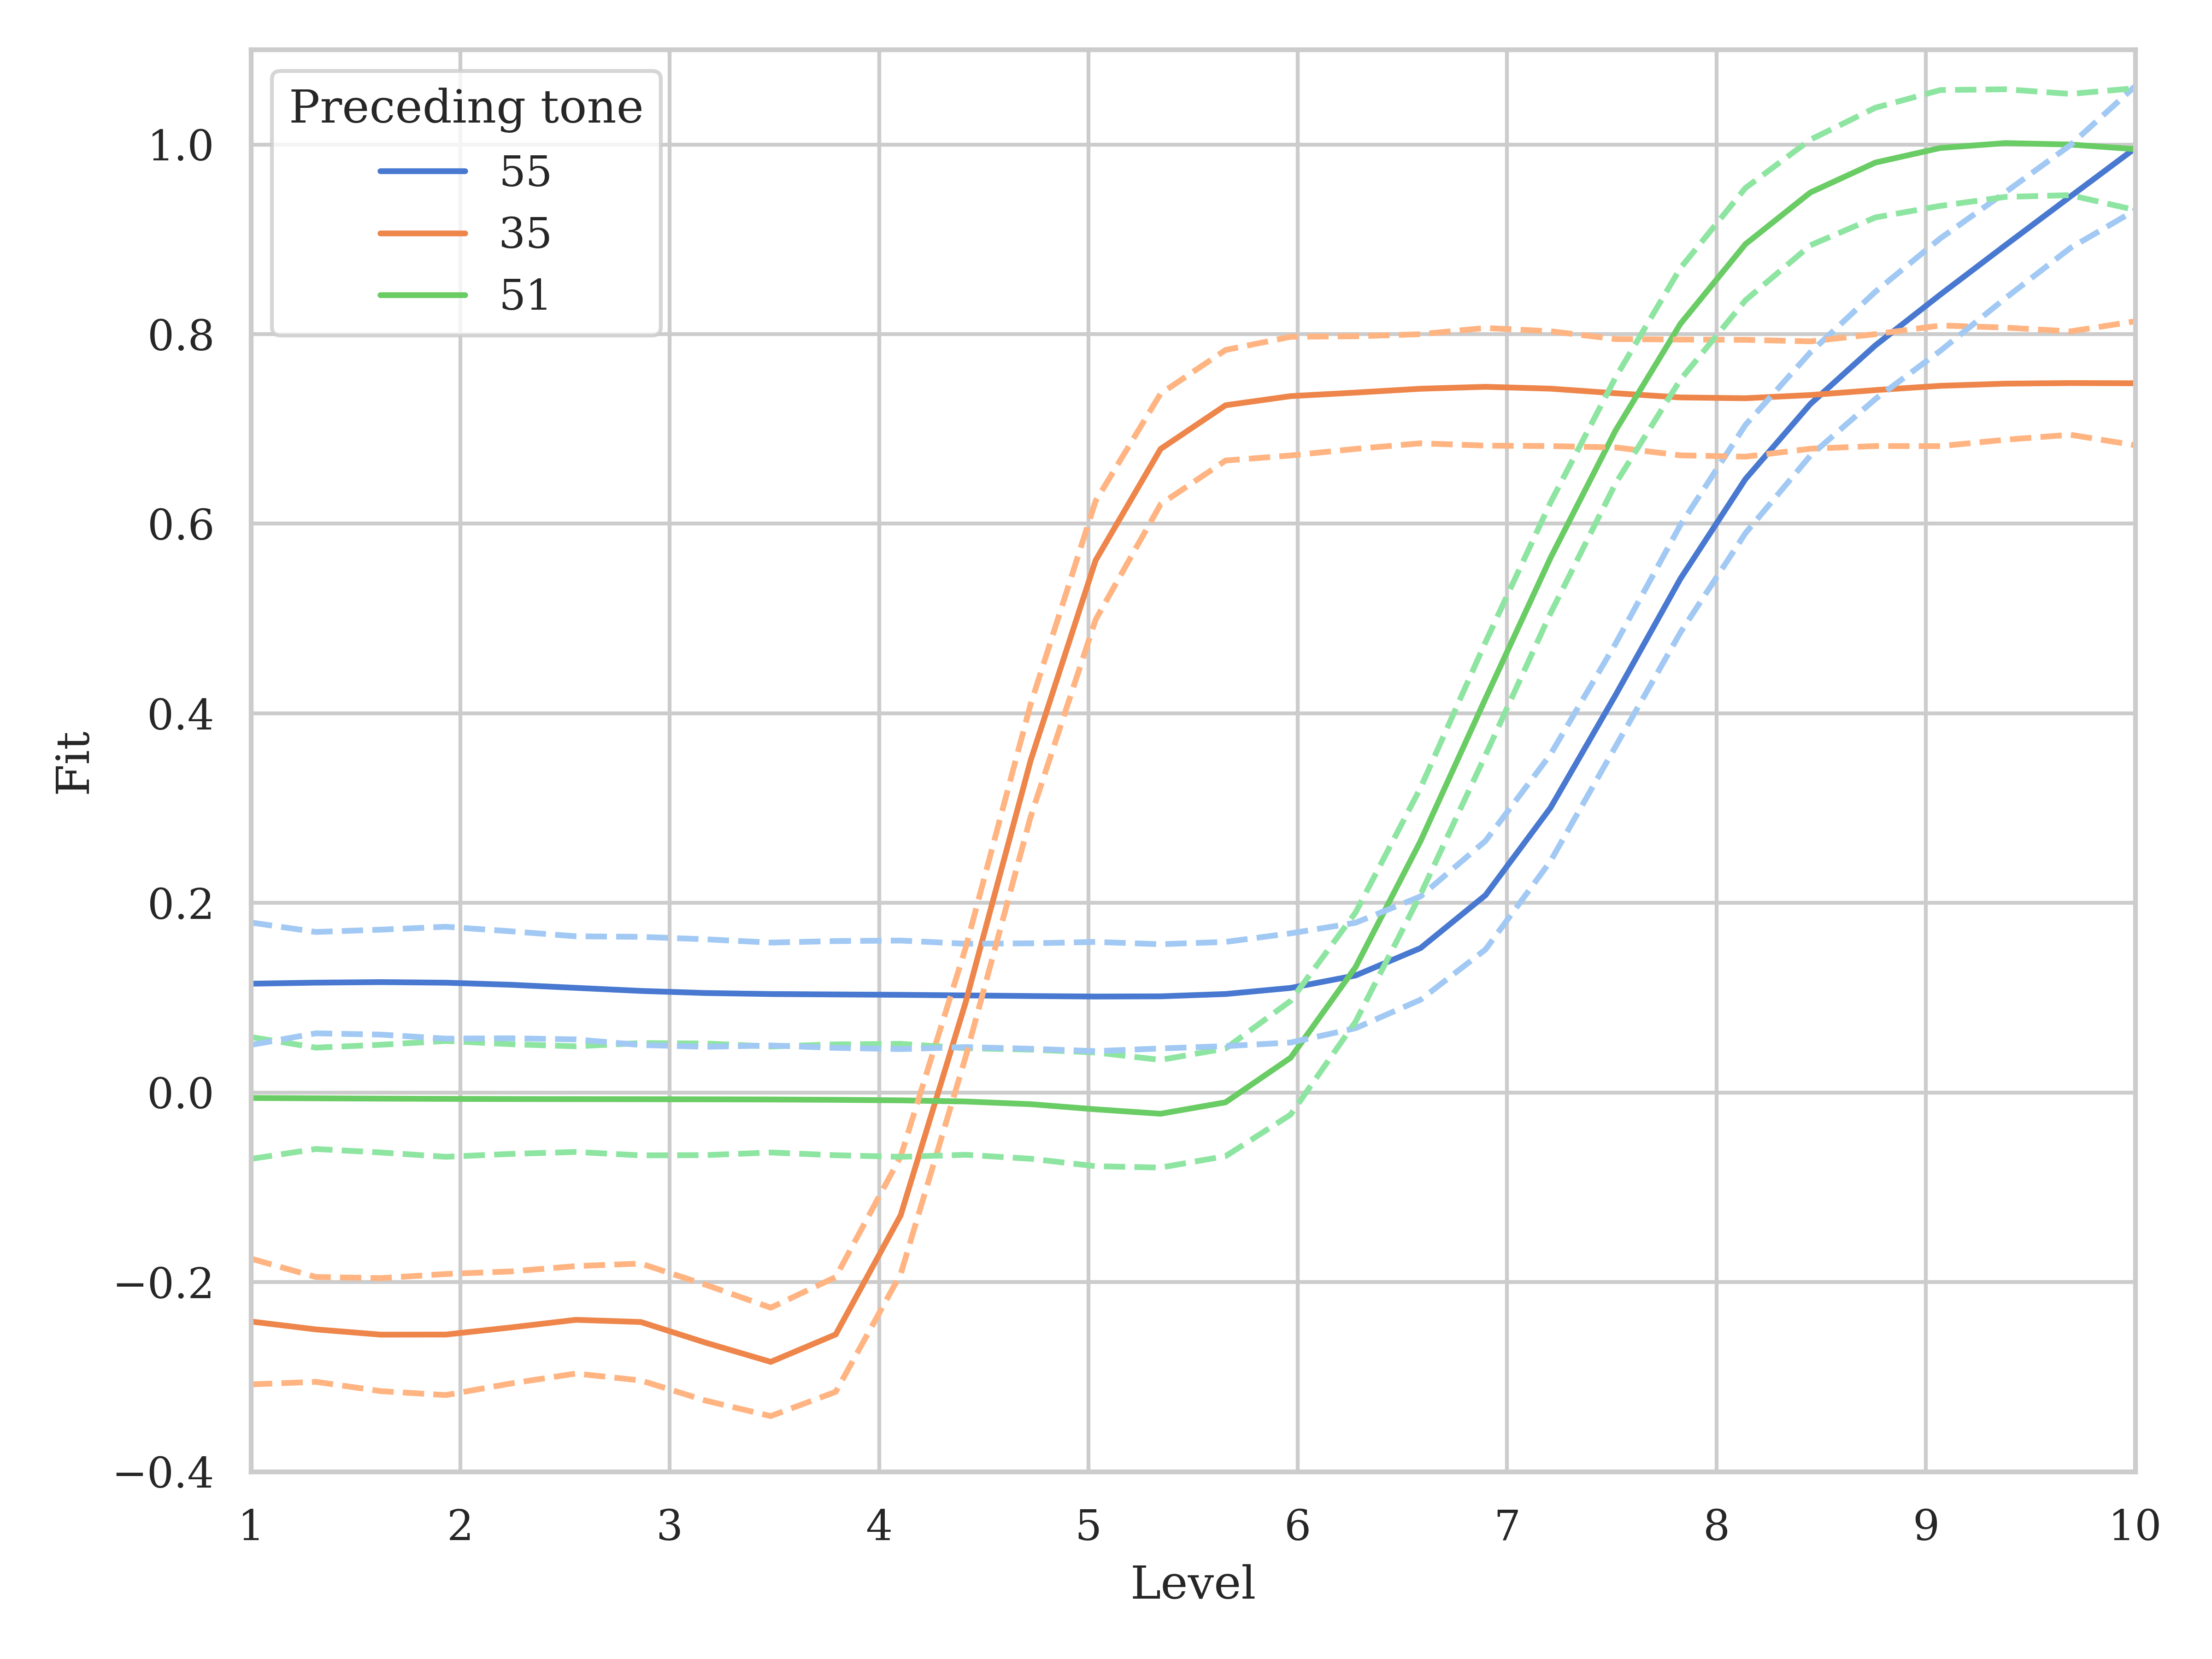
\includegraphics[width=\textwidth]{figures/E2/Mandarin_GAMM.png}
\end{subfigure}
\hfill
\begin{subfigure}[b]{.45\textwidth}
\centering
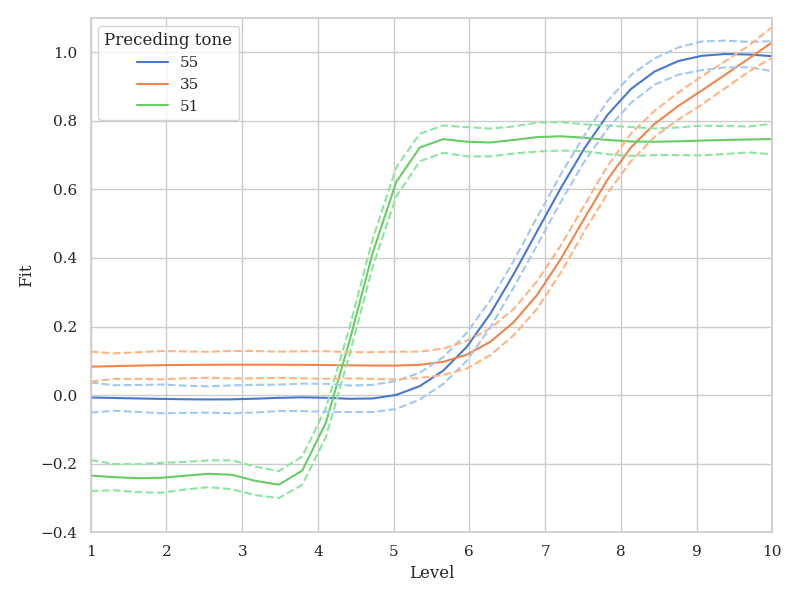
\includegraphics[width=\textwidth]{figures/E2/Mandarin_bilingual_GAMM.png}
\end{subfigure}
\hfill
\begin{subfigure}[b]{.45\textwidth}
\centering
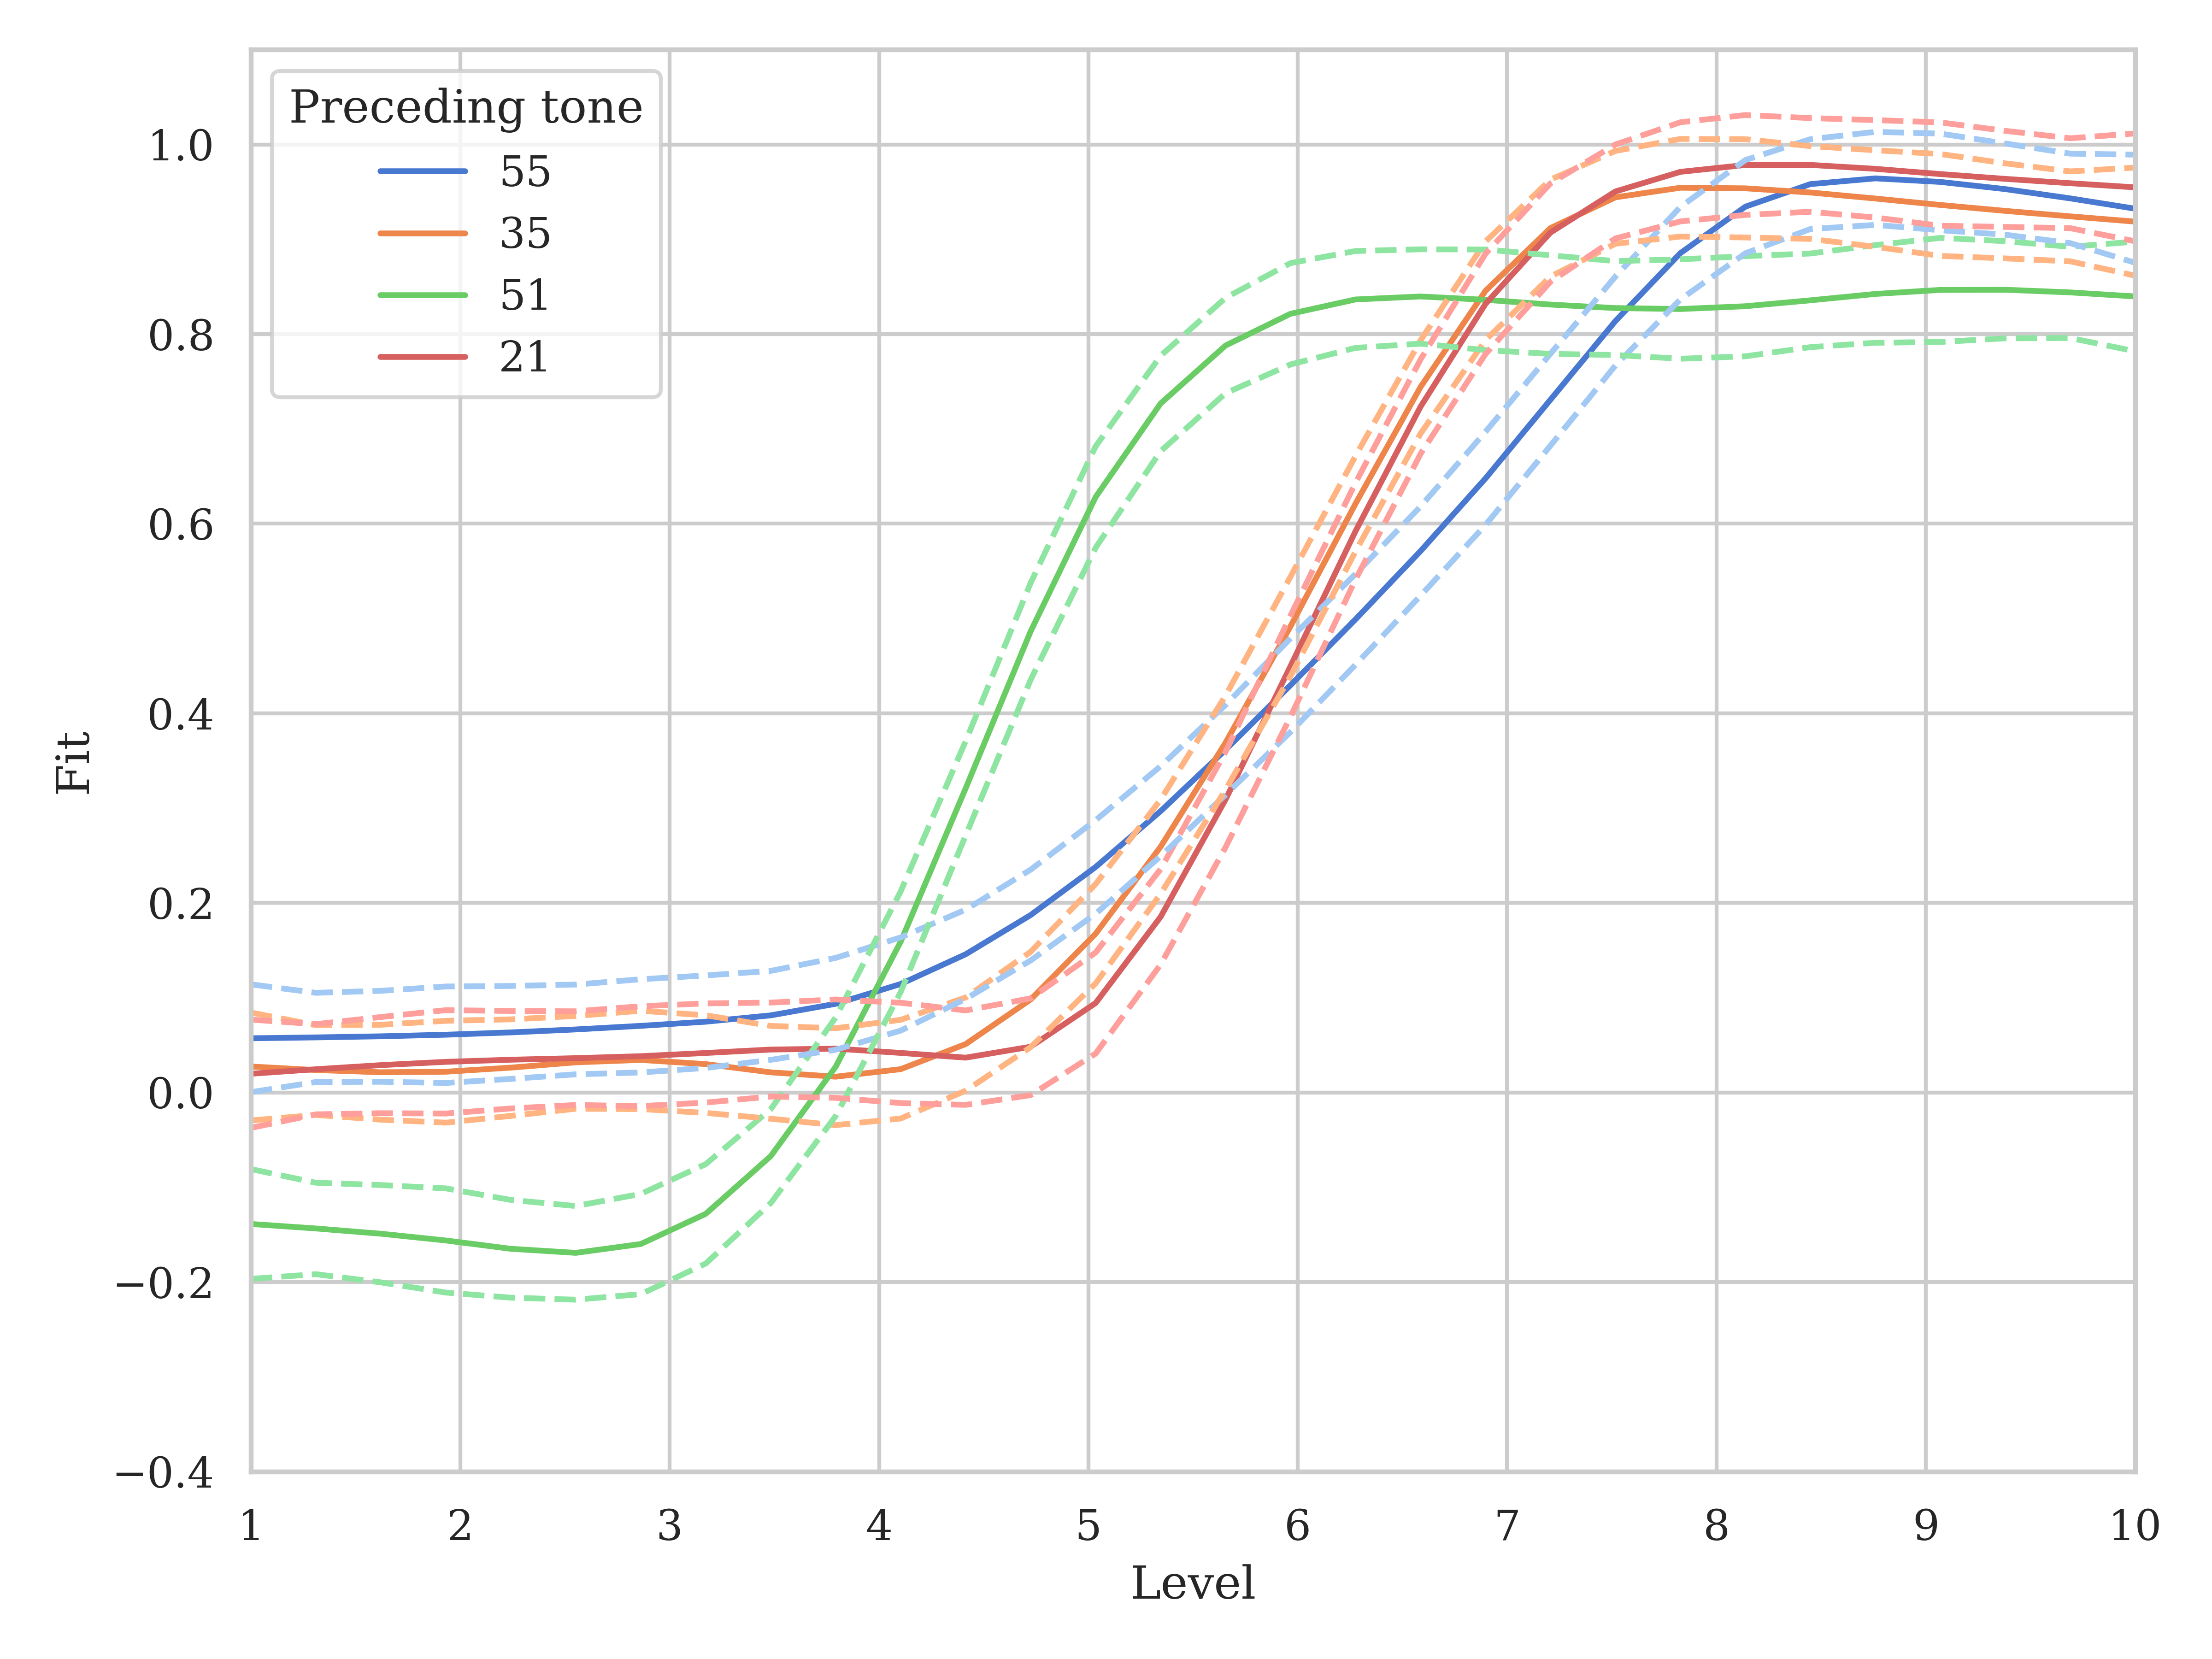
\includegraphics[width=\textwidth]{figures/E2/Min_GAMM.png}
\end{subfigure}
\caption{GAMM fitted falling tone response percentages in Experiment 2 (top left: Mandarin (monolingual); top right: Mandarin (bilingual); bottom: Southern Min).}
\label{Figure:E2GAMM}
\end{figure}

As mentioned in Section \ref{section:Experiment2}, this measurement serves as a means of quantification of the magnitudes of perceptual normalization for tonal coarticulation. The results suggest that normalization for tonal coarticulation was of a smaller amplitude in Taiwan Southern Min than in Taiwan Mandarin, and this difference between Mandarin and Southern Min, interestingly, was present not only between groups, but also within the bilingual subjects.

\section{Tone boundaries between the low tone and the falling tone in Mandarin and Taiwan Southern Min}

Raw acceptance rates of the falling tone and the low tone in Mandarin and Southern Min of the monolingual and bilingual groups are shown in Figure \ref{Figure:E3Raw}.

\begin{figure}[hbt!]
\centering
\begin{subfigure}[b]{.45\textwidth}
\centering
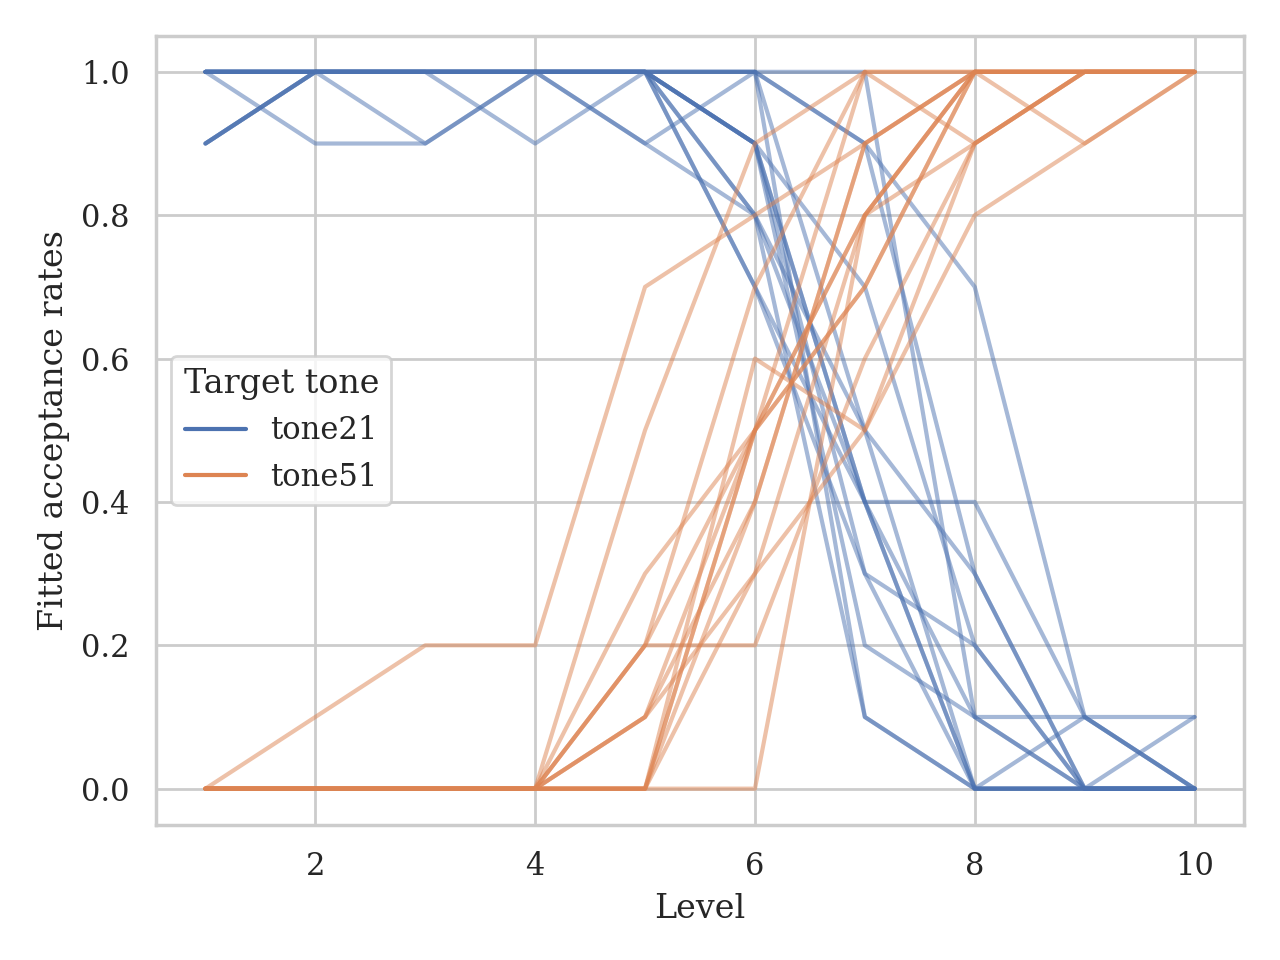
\includegraphics[width=\textwidth]{figures/E3/Mandarin_monolingual_E3_raw.png}
\end{subfigure}
\hfill
\begin{subfigure}[b]{.45\textwidth}
\centering
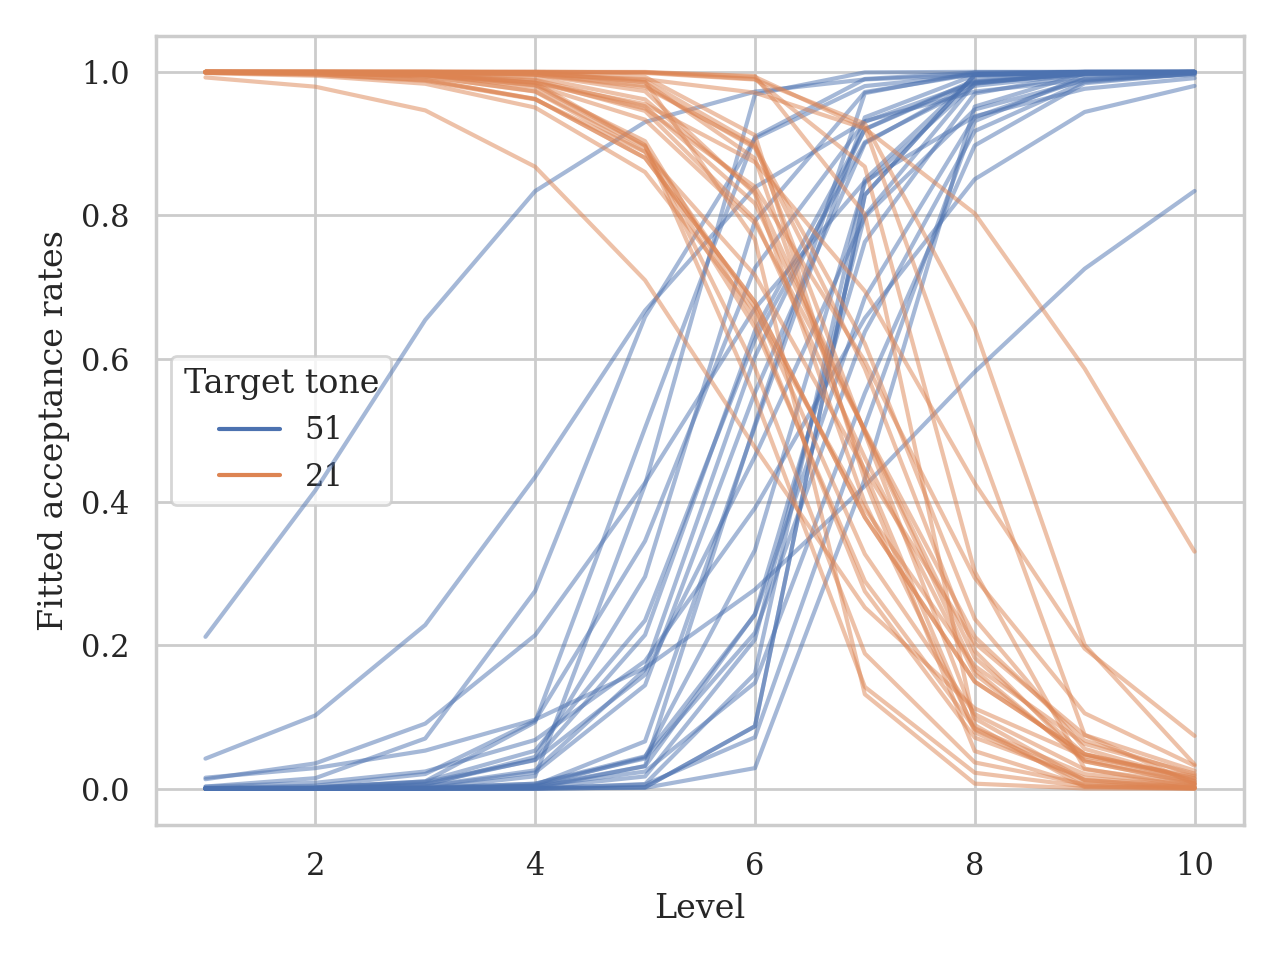
\includegraphics[width=\textwidth]{figures/E3/Mandarin_bilingual_E3_raw.png}
\end{subfigure}
\hfill
\begin{subfigure}[b]{.45\textwidth}
\centering
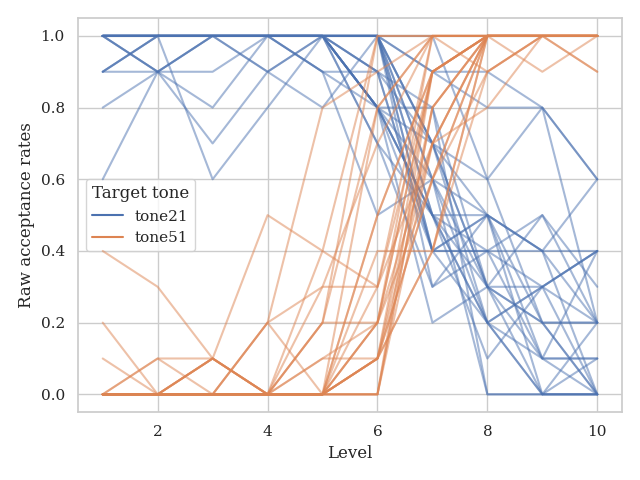
\includegraphics[width=\textwidth]{figures/E3/Min_E3_raw.png}
\end{subfigure}
\caption{Acceptance rates in Experiment 3 (top left: Mandarin (monolingual); top right: Mandarin (bilingual); bottom: Southern Min).}
\label{Figure:E3Raw}
\end{figure}

GAMM fitted first derivatives of the acceptance rates are shown in Figure \ref{Figure:E3GAMM}. It is seen that, rather straightforwardly, the falling tone acceptance rates had both higher maximum of first derivatives and higher threshold level in Taiwan Southern Min than in Taiwan Mandarin, while for the low tone, such pattern seemed absent. Simple t-tests showed that the falling tone acceptance rates in Taiwan Southern Min had substantially larger maximum of first derivatives of the acceptance rates (p=.019*), and marginally significantly higher level of threshold (p=.059). This pattern was more obvious on the advanced bilingual group (p=.005***/.091**, respectively). This pattern, however, was not seen for the low tone, where the maximum of first derivatives of the acceptance rates was higher in Taiwan Mandarin than in Taiwan Southern Min (p=.018*), and the levels of thresholds were not significantly different (p=.974).

As suggested in Section \ref{section:E3 Analyses}, the maximum of the first derivates of the acceptance rates and the level of threshold were taken as how strict the tone boundary of the target tone was in the language.
\begin{figure}[hbt!]
\centering
\begin{subfigure}[b]{.45\textwidth}
\centering
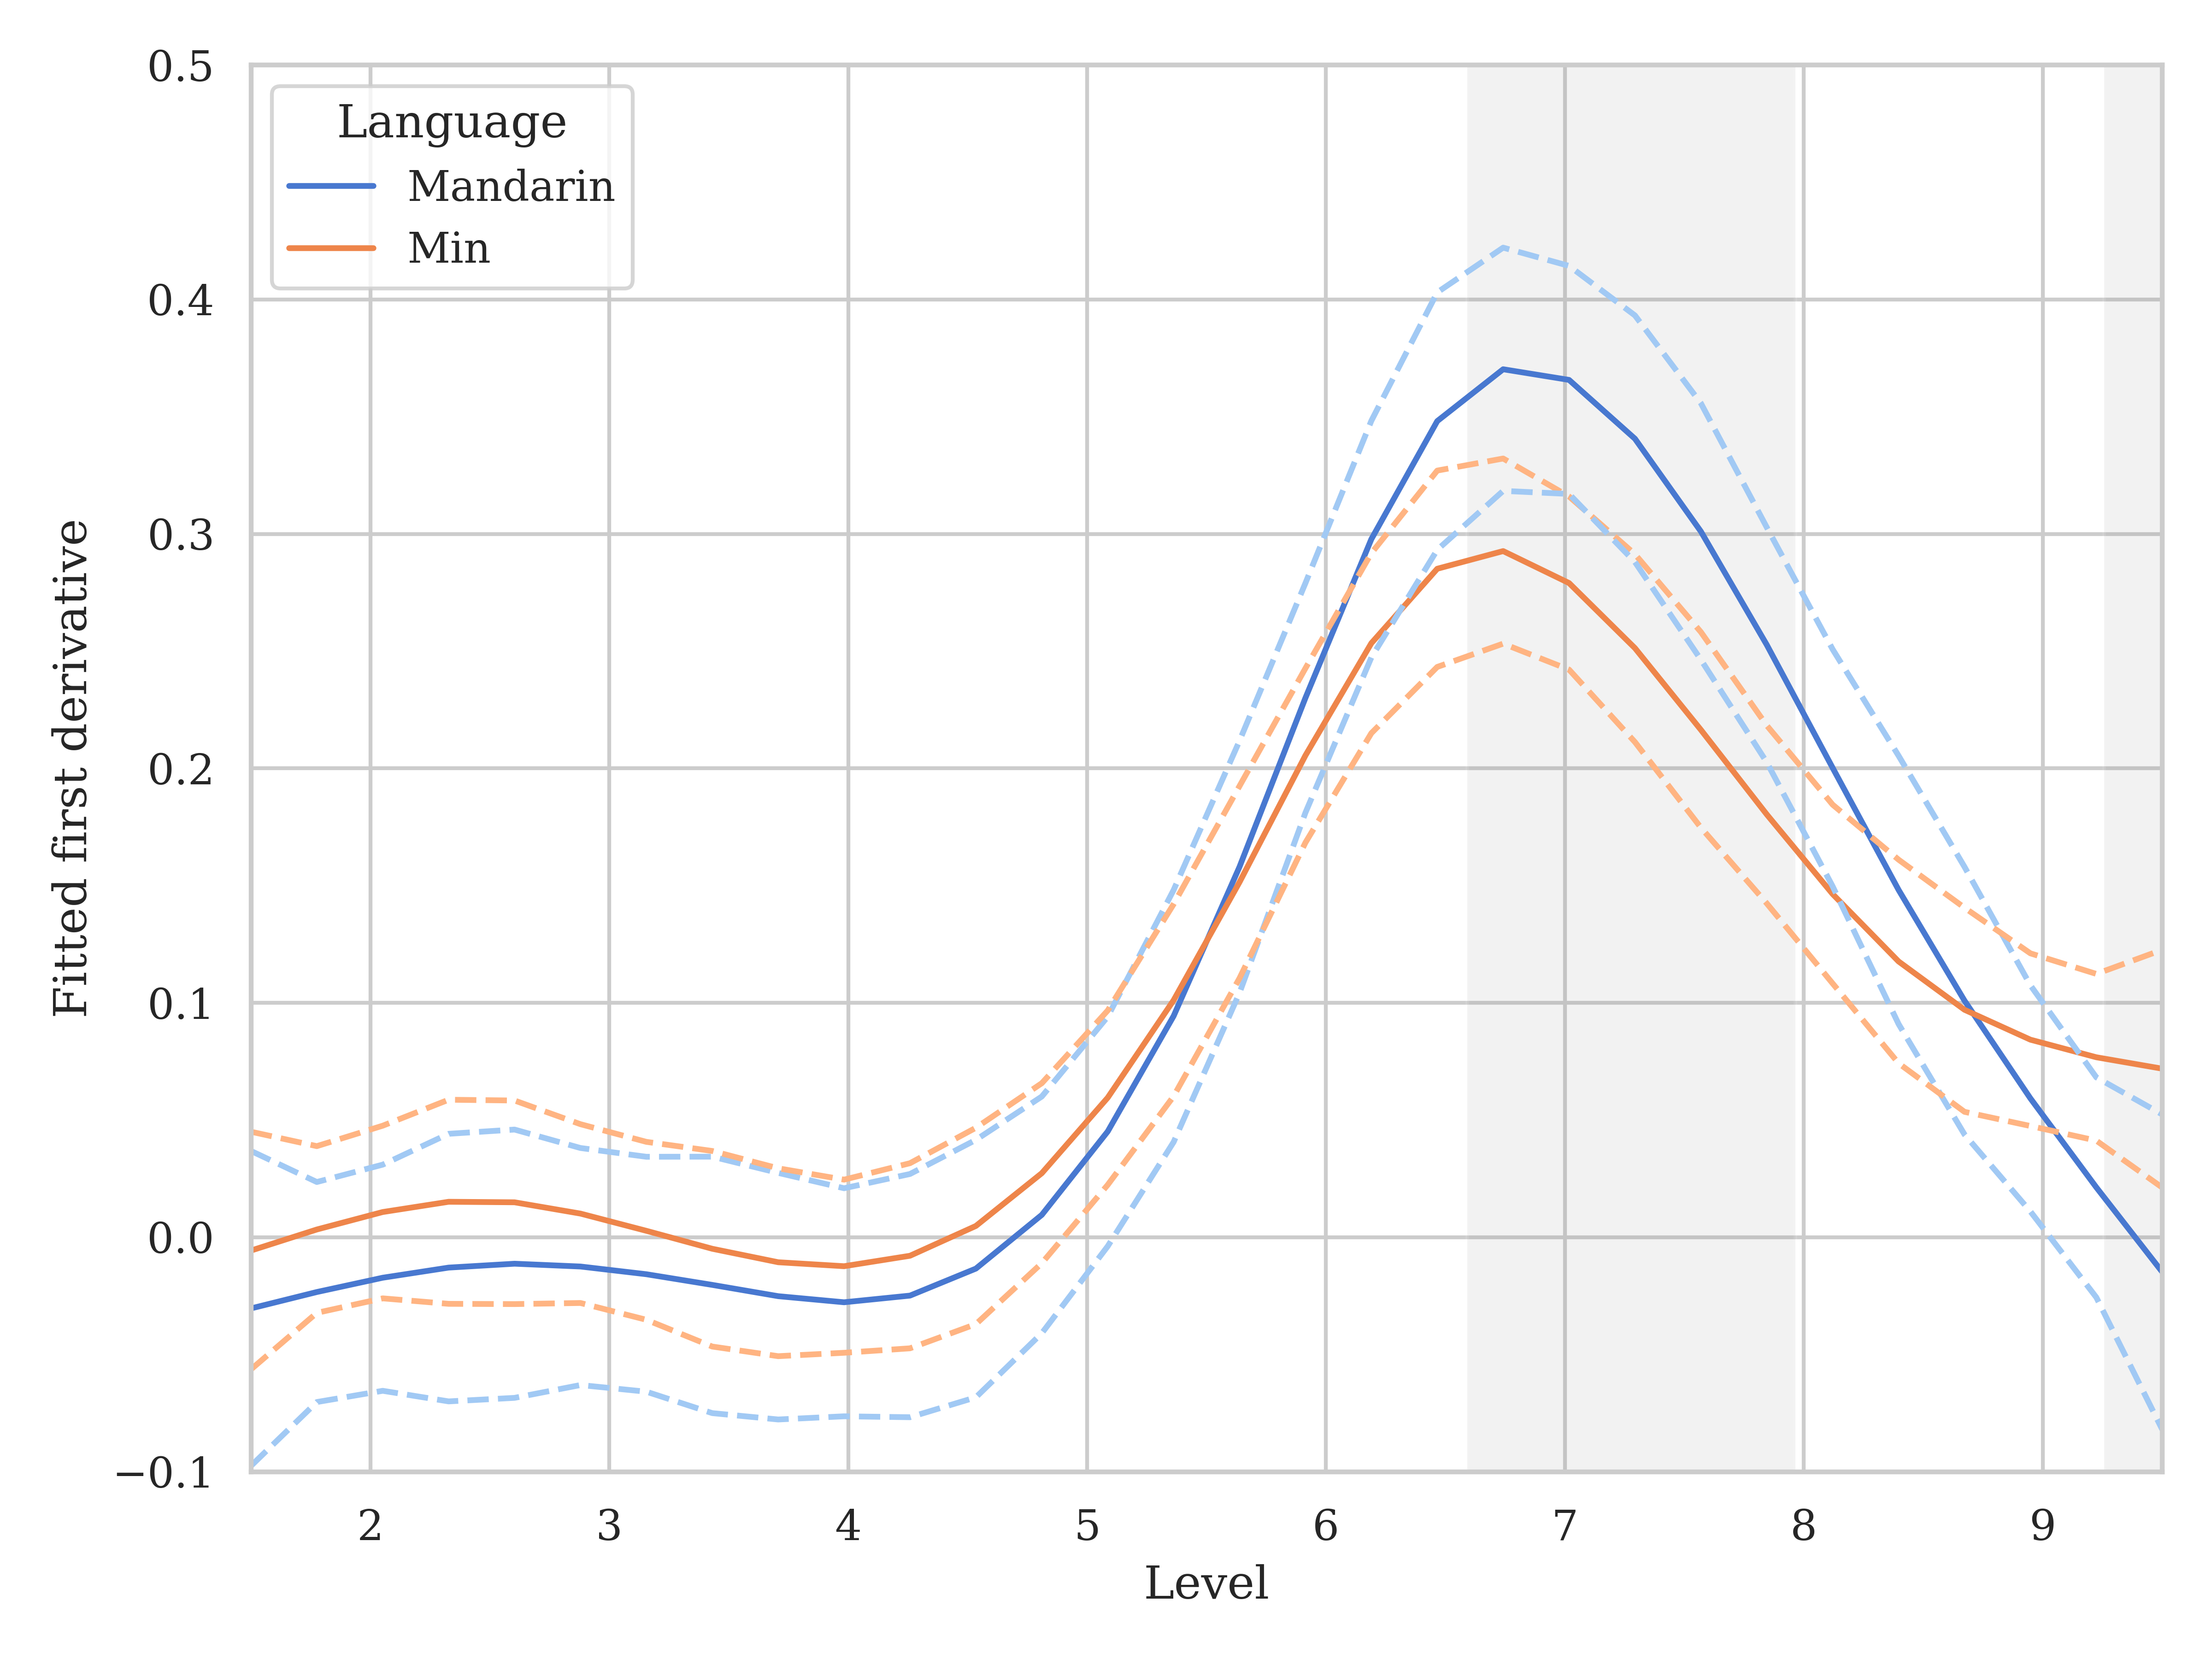
\includegraphics[width=\textwidth]{figures/E3/Tone21_speed_GAMM.png}
\end{subfigure}
\hfill
\begin{subfigure}[b]{.45\textwidth}
\centering
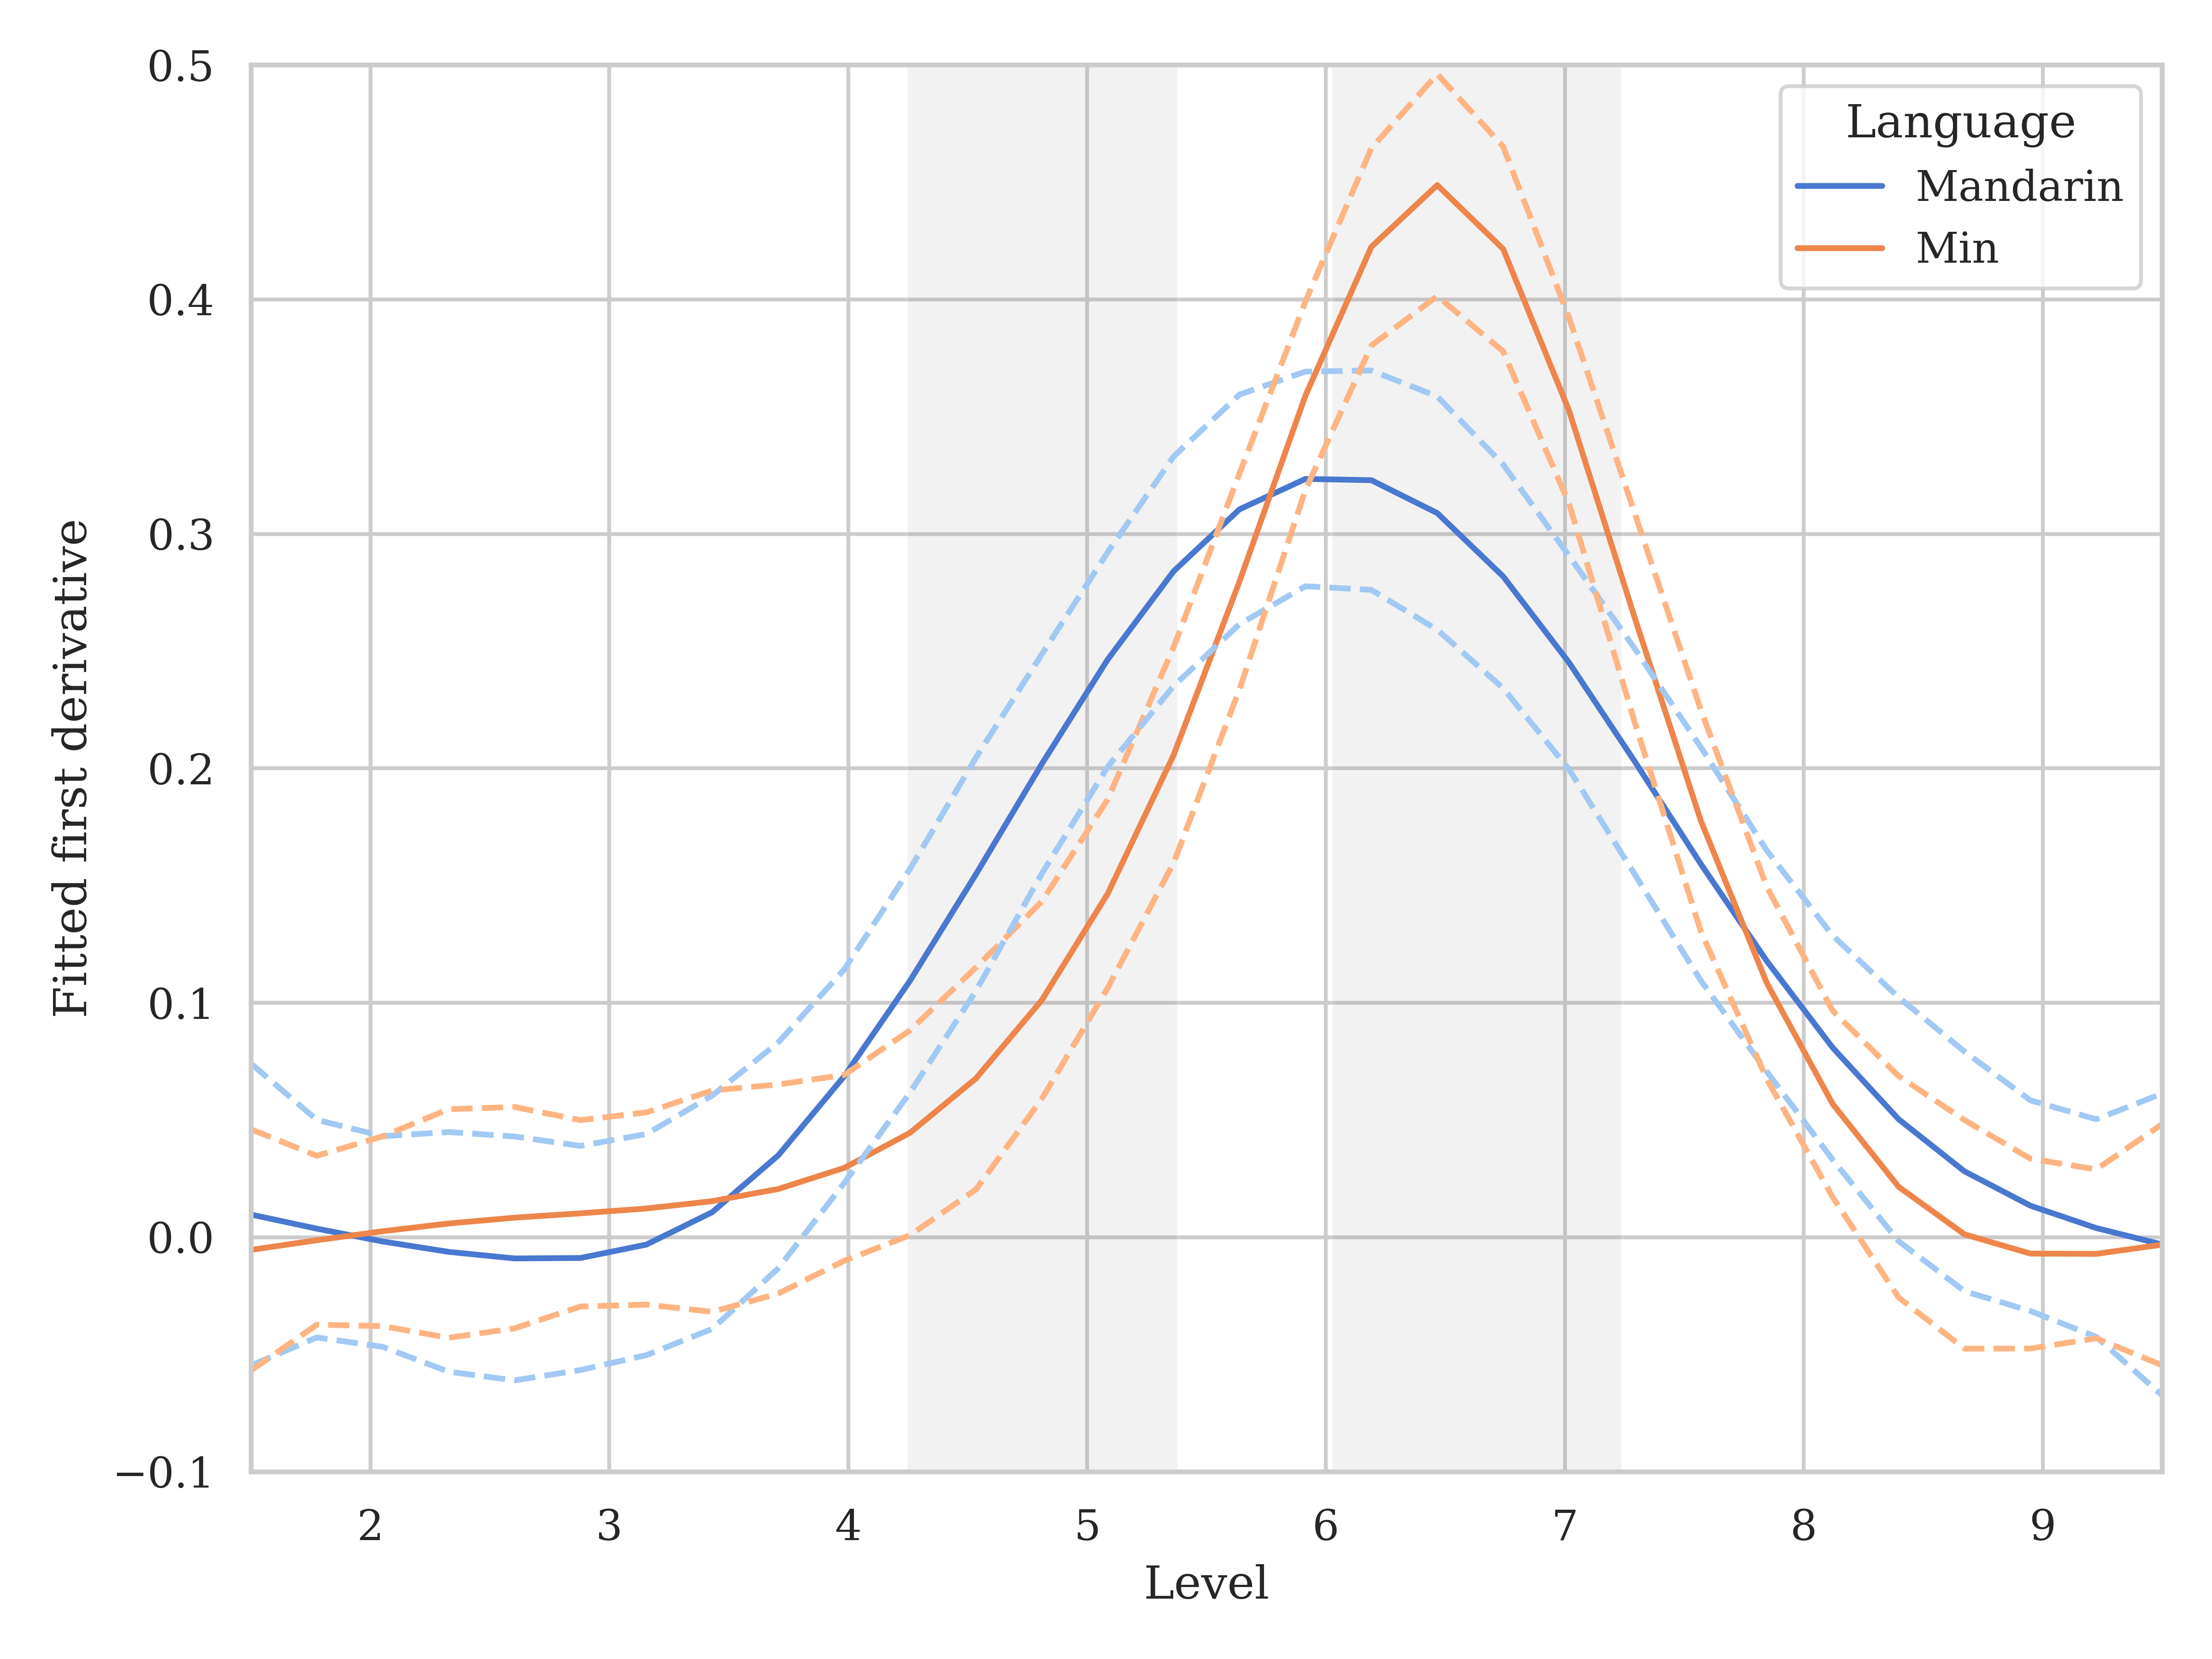
\includegraphics[width=\textwidth]{figures/E3/Tone51_speed_GAMM.png}
\end{subfigure}
\caption{GAMM fitted first derivatives of acceptance rates in Experiment 3 (left: low tone; right: falling tone). The gray areas indicate intervals of significant differences.}
\label{Figure:E3GAMM}
\end{figure}
The results suggested that the boundary was stricter in Taiwan Southern Min for the falling tone, while for the low tone, this pattern was absent. Nevertheless, we shall argue in section \ref{section:Tone boundaries and perception of tonal coarticulation} that such absence of a stricter boundary for the low tone in Taiwan Southern Min was likely due to tone sandhi rules, and that tone boundaries in general shall be deemed as stricter in Taiwan Southern Min than in Taiwan Mandarin.

As can be seen in Figure \ref{Figure:E3GAMM_bilingual}, again, the linguistic difference was seen within the bilingual subjects. Paired t-tests of within-subject comparisons of the bilingual group showed that for the falling tone, while the maximum of first derivatives of the acceptance rates was not significantly larger in Taiwan Mandarin (p=.158), the threshold was higher (i.e., closer to the right end; p=.0098***). For the low tone, the maximum of first derivatives of the acceptance rates was substantially larger in Taiwan Mandarin than in Taiwan Southern Min (p=.004**), while the threshold was not significantly different (p=.620).

\begin{figure}[hbt!]
\centering
\begin{subfigure}[b]{.45\textwidth}
\centering
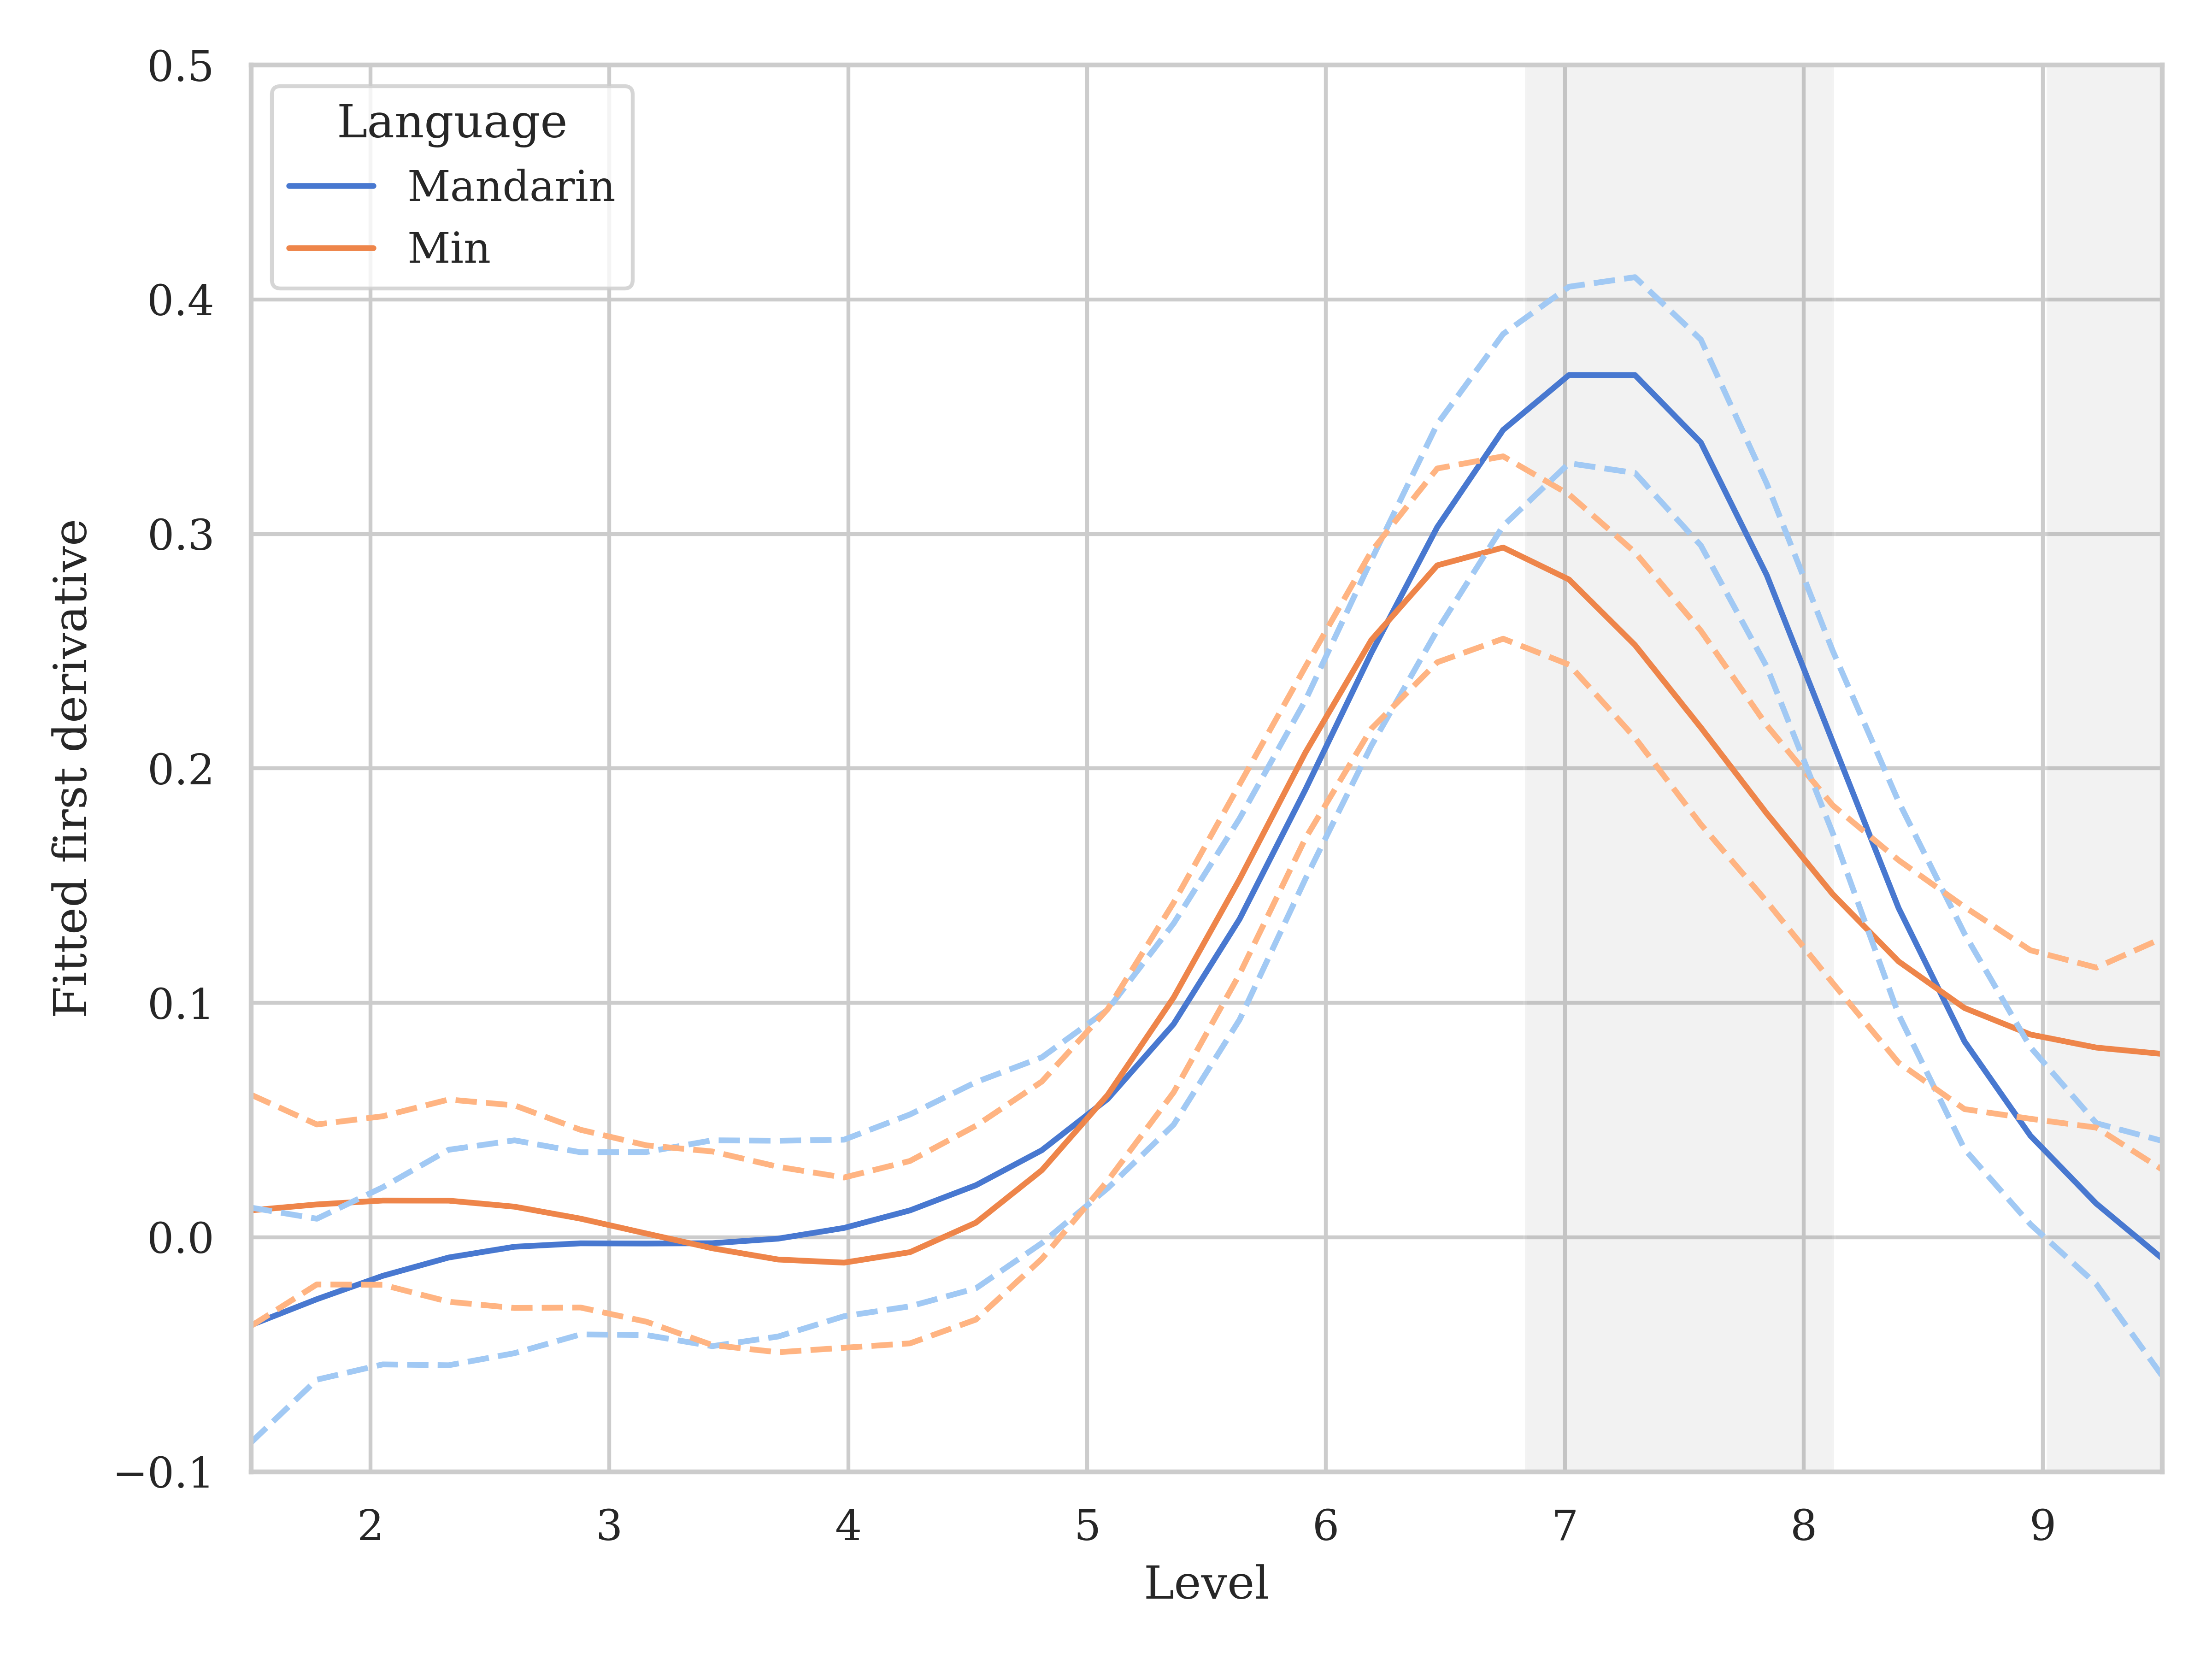
\includegraphics[width=\textwidth]{figures/E3/Tone21_speed_GAMM_bilingual.png}
\end{subfigure}
\hfill
\begin{subfigure}[b]{.45\textwidth}
\centering
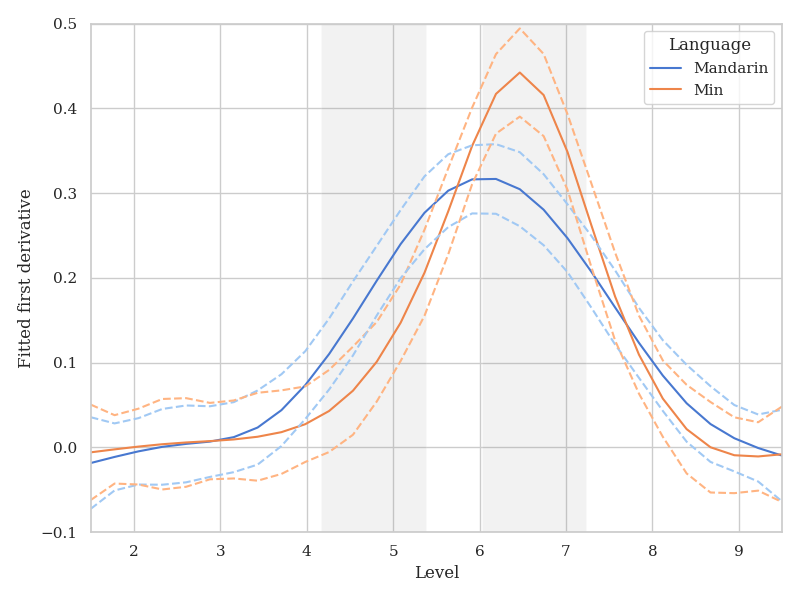
\includegraphics[width=\textwidth]{figures/E3/Tone51_speed_GAMM_bilingual.png}
\end{subfigure}
\caption{GAMMs fitted first derivatives of acceptance rates in Experiment 3 (within bilingual groups; left: low tone; right: falling tone). The gray areas indicate intervals of significant differences.}
\label{Figure:E3GAMM_bilingual}
\end{figure}

\section{Summary}
In this section, we have examined tonal coarticulation in Taiwan Mandarin and Taiwan Southern Min, and normalization and tone boundaries in the two languages. It is seen that while Taiwan Mandarin and Taiwan Southern Min exhibited rather similar distribution in terms of tonal coarticulation, Taiwan Southern Min was shown to be less influenced by the normalization effect of tonal coarticulation. Tone boundaries of the falling tone and the low tone in these two languages were also shown to be different in terms of strictness. In the next chapter, we will discuss the significances of these discrepancies and of other results that we have seen in this section.